\documentclass[titlepage, 11pt]{book}
\usepackage[utf8]{inputenc}
\usepackage[a4paper, top=3cm, bottom=3cm, left=2.5cm, right=2.5cm]{geometry}
\usepackage[spanish,activeacute,es-tabla]{babel}
\usepackage[
  backend=biber,
  style=ieee,
  giveninits=true    % Iniciales en lugar de nombres completos (opcional)
]{biblatex}
\addbibresource{TFGBib.bib}
\usepackage{float}
\usepackage{parskip}
\usepackage{graphicx}
\usepackage{amsmath, amsthm, amssymb}
\usepackage{caption, subcaption}
\usepackage{xcolor}
\usepackage{booktabs}
\usepackage{csquotes}
\usepackage{emptypage}
\usepackage{multicol}
\usepackage{titling}
\usepackage{setspace}
\usepackage[colorlinks=true, linkcolor=blue, citecolor=red, urlcolor=blue]{hyperref}

\setstretch{1.15}



\begin{document}

\pagenumbering{roman}

\begin{titlepage}
    \centering

    
\includegraphics[width=0.4\textwidth]{solemne_color.png}\par
    
    \vspace{0.5cm}
    
    {\Large\textbf{Trabajo de Fin de Grado}}\par
    {\Large Grado en Física}\par

    \vspace{0.5cm}

    \rule{\textwidth}{0.5pt}
    \vspace{0.5cm}
    {\huge\bfseries MACHINE LEARNING:\\ Métodos de ensamble aplicados a la estimación de la temperatura crítica en materiales superconductores}
    \vspace{0.5cm}
    \rule{\textwidth}{0.5pt}

    \vspace{0.5cm}
    
    {\LARGE\bfseries Marcos Barba Ballarín}\par
    \vspace{0.5cm}
    {\large Director: Ricardo López Ruiz}

    \vspace{1cm}
    
    {\large Zaragoza, \today}\par

    \vspace{1.5cm}

    
\includegraphics[width=0.4\textwidth]{facultad_ciencias-01.pdf}\par\vspace{2cm}
\end{titlepage}

\cleardoublepage

\thispagestyle{empty} % sin número de página
\vspace*{\fill}         % espacio para centrar verticalmente
\begin{flushright}
    \textit{A José Luis Ballarín,\\que espero se sintiera orgulloso.}
\end{flushright}
\vspace*{\fill}
\cleardoublepage

\chapter*{Agradecimientos}
    \addcontentsline{toc}{chapter}{Agradecimientos}
    Este proyecto supone la culminación de una etapa que, con sus altibajos, ha conformado quién soy hoy más que ninguna otra. Recuerdo el día que atravesé por primera vez las puertas de la Universidad de Zaragoza y me enfrenté a mi primera sesión de clases como uno de los mayores golpes de realidad que he recibido: por primera vez, no había podido seguir al completo la explicación de un profesor, y esto se repitió durante la mayoría de las sesiones de aquella semana y las que vendrían posteriormente. La primera reacción que emergió de mi subconsciente fue la de abandonar, nunca había sido muy fuerte en ese aspecto, y en el pasado, si algo me había supuesto demasiado esfuerzo, simplemente había huido de allí.

    Aquellos meses y en realidad, en varias ocasiones durante los dos primeros cursos, apareció esta idea en mi cabeza. Dado que hoy me encuentro escribiendo estas palabras, siento la necesidad de manifestar mi agradecimiento a varias personas, cuyo apoyo, soporte o simple presencia lo ha hecho posible.
    
    A mis padres, que nunca dejaron de confiar en mí, y me mostraron su apoyo incondicional, fueran cuales fueran las circunstancias. En ocasiones pienso que ni siquiera escuchaban cuando intentaba argumentarles la difícil situación en la que me encontraba (cegado por el agobio de los exámenes) y sencillamente me respondían: ``inténtalo, y si no, pues a la siguiente''.

    A mi hermana, con la que en cierto modo he compartido este camino universitario. La infinidad de charlas sobre lo <<jodidos que estábamos>>, en las que intentábamos quitarle importancia respectivamente a nuestras situaciones, me daban el empujón que necesitaba para pelear un poco más. Después de tanto luchar, las personas se hacen de acero, por eso estoy seguro de que conseguirás el éxito que persigues.
    
    A mis abuelas, que creyeron siempre en su nieto, aunque no estaba de más encender una vela par pedir una pequeña ayuda del cielo.

    A mis compañeros y amigos, porque con ellos he podido disfrutar de este camino. Sin ellos no habría tenido esos momentos tan necesarios para evadirme y recuperar fuerzas, mi fuente de energía estos años. Horas en la biblioteca, paradas por café, charletas en una habitación de la resi y alguna que otra noche mágica, son algunas de las experiencias que me llevo de estos años increíbles.


\chapter*{Resumen}
\addcontentsline{toc}{chapter}{Resumen}
El aprendizaje automático, ampliamente conocido por su acepción en inglés \textit{machine learning}, vive hoy una época dorada, especialmente en el área del \textit{deep learning} y las inteligencias artificiales generativas. No obstante, sin tanta repercusión mediática y antes de que estos modelos vieran la luz, las últimas décadas han estado lideradas por multitud de modelos predictivos que, sin alcanzar los increíbles resultados de las redes neuronales modernas, siguen siendo la elección preferida por muchos profesionales en ámbitos tan diversos como la investigación científica, la detección de fraude bancario, la predicción de mercados financieros o la toma de decisiones corporativas, entre otros.

En la mayoría de los casos, los modelos a los que actualmente nos referimos como \textit{machine learning} <<tradicional>>, no alcanzan los sorprendentes rendimientos de los modernos algoritmos basados en redes neuronales. Sin embargo, su estabilidad, su menor necesidad de datos e infraestructura computacional y, sobre todo, su explicabilidad, que nos permite interpretar cuál es la estrategia que el algoritmo ha encontrado para obtener las predicciones, los convierten en una opción realmente atractiva.

En el presente proyecto tomamos la iniciativa de estudiar algunos de los modelos más potentes de esta área del aprendizaje automático: aquellos algoritmos que, por medio de los conocidos como métodos de ensamble, combinan varios modelos en uno solo para lograr un mayor rendimiento. No sin antes revisar la estructura básica utilizada por todas estas técnicas: el árbol de decisión.

El objetivo será no solo acercarnos al funcionamiento de estas técnicas, sino también desarrollar una aplicación práctica, en este caso, en el ámbito de la investigación científica y, en particular, de la física de materiales: predecir la temperatura crítica en compuestos superconductores. Además, discutiremos las posibilidades que, tras el auge del \textit{deep learning}, quedan para este tipo de modelos.

\tableofcontents

\chapter{Machine Learning}
\pagenumbering{arabic}
Aprender a partir de la experiencia, una habilidad que se atribuye generalmente a los seres vivos, especialmente a los pertenecientes al mundo animal y, en particular, a los seres humanos, es una de las características fundamentales que componen la inteligencia. Desde los inicios de la computación, se ha perseguido el objetivo de dotar a las máquinas de esta capacidad, en una constante búsqueda de alcanzar algún grado de \textbf{inteligencia artificial}.

El aprendizaje automático \textit{(Machine Learning)} constituye un ámbito dentro de esta disciplina y hace referencia al conjunto de métodos y algoritmos que permiten que un sistema aprenda relaciones y patrones de forma autónoma, optimizando su funcionamiento con el objetivo de minimizar el error cometido en sus predicciones, a este proceso en el que el modelo <<aprende>> de la información que se le proporciona lo llamamos \textbf{entrenamiento}.

En función de los datos disponibles para el entrenamiento de un modelo, es posible distinguir dos tipos de aprendizaje: \textbf{supervisado} y \textbf{no supervisado}.

\section{Tipos de aprendizaje}
El \textbf{aprendizaje supervisado} es aquel en el que el conjunto de datos incluye ejemplos de entrada junto con sus correspondientes salidas o etiquetas. El objetivo es que el modelo aprenda las relaciones subyacentes entre ambas, de modo que, ante nuevas entradas para las cuales no se dispone de salida real, sea capaz de realizar una predicción adecuada. En función del tipo de variable que constituya la salida, los problemas pueden clasificarse como de \textbf{regresión}, cuando la salida es una variable numérica continua, o de \textbf{clasificación} cuando la salida es discreta y el modelo debe asignar cada muestra a una categoría o etiqueta determinada.

En contraste, el \textbf{aprendizaje no supervisado} se emplea cuando los datos no cuentan con etiquetas ni valores objetivo. Los modelos buscan descubrir estructuras o patrones subyacentes en los datos, agrupando observaciones similares o reduciendo la dimensionalidad del conjunto. Los algoritmos de \textit{clustering} como \textit{K-Means}, o los métodos de reducción de dimensionalidad como el \textit{Análisis de Componentes Principales (PCA)} son ejemplos de aprendizaje no supervisado.

En el presente estudio vamos a centrarnos en técnicas de \textbf{aprendizaje supervisado}, dado que constituye el enfoque más adecuado para problemas de predicción en los que disponemos de ejemplos con salida conocida. En concreto, profundizaremos en los modelos de \textbf{árboles de decisión} y en sus principales técnicas de ensamble.

\section{División del conjunto de datos} \label{sec:div_dataset}
En el aprendizaje supervisado es habitual dividir el conjunto de datos en dos partes: \textbf{entrenamiento} y \textbf{test}. El primero se utiliza durante el aprendizaje del modelo, es de este subconjunto del que el modelo extrae las relaciones y patrones subyacentes. El segundo se utiliza para evaluar la capacidad del modelo de generalizar a datos nunca antes vistos y determinar su capacidad predictiva.

Esta separación resulta esencial para evitar el \textbf{sobreajuste} \textit{(overfitting)}, es decir, que el modelo memorice los ejemplos de entrenamiento y pierda capacidad predictiva sobre información nueva.

Generalmente, entre un $70\%$ y un $80\%$ de los datos se destinan al entrenamiento, y el resto al test, aunque la proporción puede variar dependiendo del tamaño del conjunto de datos disponible.

\section{Hiperparámetros}
Como ya se ha mencionado, son los propios modelos los que ajustan de forma autónoma sus parámetros internos, adaptándose al conjunto de entrenamiento que se les proporciona. No obstante, los modelos de aprendizaje automático cuentan, en general, con una serie de parámetros externos denominados \textbf{hiperparámetros} que determinan su comportamiento y complejidad.

Estos parámetros deben fijarse previo al entrenamiento y su elección resulta crucial para el correcto funcionamiento del modelo, pues condicionará su capacidad de ajuste y generalización. Hiperparámetros mal seleccionados pueden derivar en modelos con exceso de \textbf{sesgo} o \textbf{varianza}. Usualmente, son seleccionados mediante pruebas sucesivas en las que se modifican sus valores hasta encontrar la combinación que proporciona el rendimiento óptimo del modelo.

\section{Evaluación del modelo}
Durante todo este capítulo se ha estado haciendo referencia a la evaluación del rendimiento del modelo, algo fundamental para cuantificar la capacidad de este de generalizar a nuevos datos. No obstante, todavía no habíamos profundizado en cuáles son las herramientas para llevar a cabo esta tarea.

La \textbf{validación} tradicional es una evaluación sobre el subconjunto de test, introducido en la sección \ref{sec:div_dataset}. El modelo se ajusta en primer lugar utilizando el subconjunto de entrenamiento, y se evalúa su rendimiento con el subconjunto de test. De esta forma analizamos su funcionamiento con datos no vistos durante el entrenamiento. La principal limitación de este método es que la evaluación depende de una única división del conjunto de datos, lo que puede introducir cierta variabilidad.

Para mitigar este problema se recurre a \textbf{validación cruzada} \textit{(cross-validation)} y, en particular, a su procedimiento más habitual: \textit{k-fold cross-validation}. El conjunto de datos se divide en $k$ particiones o \textit{folds} de tamaño similar. El modelo se entrena $k$ veces, utilizando en cada iteración $k-1$ particiones para el entrenamiento y la restante para validación. Las métricas de evaluación se obtienen como la media de las obtenidas en cada validación. El resultado es una estimación más estable y representativa del rendimiento real del modelo.

Habitualmente, \textit{cross-validation} se utiliza como una fase previa al entrenamiento final del modelo. Su propósito es obtener una estimación preliminar del rendimiento y optimizar hiperparámetros.

\chapter{Árboles de decisión}
En este capítulo se van a tratar los métodos de \textit{machine learning} basados en árboles, tanto para problemas de regresión como de clasificación. La metodología se basa en la segmentación del espacio de predictores en regiones más simples y homogéneas. El objetivo es lograr estimaciones para cada región, basándonos en las variables respuesta de las muestras de entrenamiento que pertenecen a dicha región \cite{ISLP}.

Todos estos métodos de partición del espacio pueden representarse mediante una estructura en forma de árbol. Las divisiones vienen dadas por nodos, donde se establecen condiciones basadas en los predictores. El resultado son una serie de nodos terminales u hojas, que representan cada una de las regiones segmentadas \cite{ISLP}.


\section{Entrenamiento del árbol} \label{sec:TreeTrain}
Ahora debemos tratar el proceso de construcción de un modelo de árbol. Como ya se deja entrever en la introducción, nos encontramos con dos desafíos clave \cite{ISLP}:
\begin{itemize}
    \item División del espacio de predictores, dado por el conjunto de vectores de observaciones \(X_i, i=1,\ldots,l\), en \(K\) regiones independientes \(R_1, R_2, \ldots, R_K\).
    \item Determinar una predicción para cada región $R_k, k=1,\ldots,K$, basándonos en las variables respuesta de las observaciones de entrenamiento en $R_k$
\end{itemize}

La estrategia seguida para que sea computacionalmente asumible entrenar árboles se denomina \textit{Recursive binary splitting}, explicada por \cite{CART}.

\subsection*{\textit{Recursive binary splitting}} \label{subsec:RecBinSplit}
Sean el conjunto de entrenamiento $\mathcal{T}= \{(X_i,y_i) \}_{i=1}^{l}$, donde $X_i \in \mathbb{R}^p$ con $p$ el número de características. Las variables respuesta son $y_i \in \mathbb{R}$ en caso de regresión y $y_i \in \mathcal{C}$ en caso de clasificación. Un árbol de decisión divide recursivamente el espacio de forma que las muestras con variables respuesta similares sean agrupadas conjuntamente.

Sea $Q_m$ el conjunto de observaciones contenidas en el nodo $m$. Para cada posible división $\theta =(j,t_m)$, parametrizada por una de las $p$ características $j$ y un umbral $t_m$, se obtienen dos subconjuntos $Q^{left}_m(\theta)$ y $Q^{right}_m(\theta)$.
\begin{equation*}
    \begin{split}
        Q^{left}_m(\theta) &= \{ (X_i,Y_i)|x_{i_j} \leq t_m \} \\
        Q^{right}_m(\theta) &= \{ (X_i,Y_i)|x_{i_j} > t_m \}
    \end{split}
\end{equation*}


Para un nodo $m$, \textit{recursive binary splitting} considera los $p$ predictores, y el posible valor umbral $t_m$ para cada predictor. Una función de impureza $\mathcal{L}()$ es la encargada de evaluar cada posible división $\theta(j,t_m)$, eligiendo la que minimiza la impureza total ponderada:
\begin{equation}
    \mathcal{I}(Q_m,\theta)= \frac{|Q^{left}_m|}{|Q_m|}\mathcal{L}(Q^{left}_m(\theta))+\frac{|Q^{right}_m|}{|Q_m|}\mathcal{L}(Q^{right}_m(\theta))
    \label{eq:ImpPond}
\end{equation}
donde se tiene en cuenta el peso ponderado de cada subconjunto. La función de impureza $\mathcal{L}()$ viene determinada por las características del problema, principalmente si se trata de regresión o clasificación.

Esta metodología puede generalizarse al caso en que un predictor es categórico. Sea una variable categórica $j$, se elige un subconjunto $S$ de categorías y el espacio de observaciones se divide según $x_{i_j} \in S$ o $x_{i_j} \notin S$.

Este algoritmo nos proporciona la división que minimiza localmente la impureza de cada división. No obstante, esta metodología no nos garantiza la obtención de la estructura óptima global para el árbol. A este tipo de estructuras se les denomina voraces (\textit{greedy}). Los algoritmos voraces son, además, muy propensos al \textit{overfitting}, en la sección \ref{sec:TreeOF} se tratarán estrategias para mitigar el problema.


\section{Árboles de regresión}
Cuando hablamos de árboles de regresión, nos referimos a aquellos que utilizamos para problemas de regresión, en los que la variable respuesta es continua.

A la hora de evaluar las posibles divisiones en un árbol de regresión, minimizamos una función de pérdida $\mathcal{L}()$. Según \cite{scikit-learn}, los criterios a utilizar son el error cuadrático medio (MSE), la desviación de Poisson y el error medio absoluto (MAE). Para el nodo $m$, que contiene un conjunto de observaciones $Q_m$, podemos calcular la función de pérdida:
\paragraph*{Error Cuadrático Medio (MSE):}
\begin{equation*}
    \mathcal{L}(Q_m)=\frac{1}{|Q_m|}\sum_{y \in Q_m}(y-\bar{y}_m)^2
\end{equation*}

\paragraph*{Desviación de Poisson:}
\begin{equation*}
    \mathcal{L}(Q_m)=\frac{1}{|Q_m|}\sum_{y \in Q_m}(y \log{\frac{y}{\bar{y}_m}}-\bar{y}_m)
\end{equation*}
siendo necesario que $y \geq 0$. Utilizar la desviación de Poisson puede ser útil cuando se trata de conteos o frecuencias.

Tanto en el caso del error cuadrático medio (MSE) como en el de la Desviación de Poisson, la predicción asignada a un nodo terminal del árbol corresponde al valor medio de las variables respuesta $y_i$ de las muestras contenidas en dicho nodo, ya que este valor minimiza la función de pérdida en ambos casos.
\begin{equation*}
    \bar{y}_m=\frac{1}{|Q_m|}\sum_{y \in Q_m}y
\end{equation*}

\paragraph*{Error Medio Absoluto (MAE):}
\begin{equation*}
    \mathcal{L}(Q_m)=\frac{1}{|Q_m|} \sum_{y \in Q_m} |y- mediana(y)_m|
\end{equation*}

Cuando usamos el error medio absoluto, para cada nodo terminal, se define como predicción la mediana $mediana(y)_m$\footnote{La mediana es el valor que divide un conjunto ordenado de datos en dos mitades con igual número de elementos.} del subconjunto $Q_m$:
\begin{equation*}
    mediana(y)_m=\underset{y \in Q_m}{mediana}(y)
\end{equation*}



\section{Árboles de clasificación}
Utilizados para afrontar problemas de clasificación, estos árboles funcionan de forma muy similar a los de regresión. La diferencia más notable es que la variable respuesta ahora es categórica. En consecuencia, no solo se requiere un método distinto para obtener la predicción en cada región, sino que necesitaremos otros criterios para construirlos.

Basándonos en \cite{scikit-learn}, existen distintos criterios que tienen el objetivo de encontrar los nodos más homogéneos/puros posibles. Sean $k=1,2,...,K$ las distintas clases que encontramos en el nodo $m$ definimos $p_{mk}$:
\begin{equation*}
    p_{mk}=\frac{1}{|Q_m|} \sum_{y \in Q_m}1\{y=k\} 
\end{equation*}
como la proporción de observaciones que pertenecen a la clase $k$ en el nodo $m$. Notar que $1\{y=k\}$ es una función indicadora, que toma el valor $1$ cuando se cumple la condición, mientras que se anula para el resto de valores.

\subsubsection*{\textit{Classification error rate:}}
Proporción de observaciones que no pertenecen a la clase mayoritaria del nodo.
\begin{equation*}
    \mathcal{L}(Q_m)=1-max_k(p_{mk})
\end{equation*}
Sin embargo, no es suficientemente sensible para crear buenos árboles, por lo que no es usualmente empleado.

\paragraph*{Índice de Gini:}
Cuantifica la impureza del conjunto en términos de la distribución de clases en este.
\begin{equation*}
    \mathcal{L}(Q_m)=Gini(Q_m)=\sum^K_{k=1}p_{mk}(1-p_{mk})
\end{equation*}
Si $\mathcal{L}(Q_m) = 0$, el nodo $m$ es completamente <<puro>>, lo que significa que todos los ejemplos en ese nodo pertenecen a la misma clase. Si $\mathcal{L}(Q_m)$ se acerca a 1, el nodo es más <<impuro>>, es decir, las muestras están más distribuidas entre las distintas clases.


\paragraph*{Entropía:}
La entropía es una forma de cuantificar el desorden de un sistema.
\begin{equation*}
    \mathcal{L}(Q_m)=Entropy(Q_m)=-\sum^K_{k=1}\hat{p}_{mk}\log(\hat{p}_{mk})
\end{equation*}
En el caso de los nodos, el desorden se relaciona estrechamente con la impureza. Cuando un nodo contiene únicamente observaciones de una clase (puro), su entropía es cero. En cambio, cuando las clases están repartidas uniformemente en el nodo (totalmente impuro), su entropía es máxima (igual a 1).

En clasificación la predicción se basa en la clase mayoritaria dentro de la región, es decir, la moda de las observaciones en cada región. De igual forma, se suele acompañar del porcentaje de cada clase en dicha región, lo que nos aporta información sobre la confianza de la predicción.
\begin{equation*}
    \bar{y}_m=\arg\max_{k} \, p_{mk}
\end{equation*}


\section{Evitar el \textit{overfitting}} \label{sec:TreeOF}
Los modelos descritos se ajustan muy bien a las observaciones de entrenamiento, reduciendo rápidamente su error asociado. Los árboles se ramifican adquiriendo estructuras complejas y generando sobreajuste \textit{(overfitting)}, perdiendo generalización. Como vemos planteado en \cite{CART}, limitar el tamaño del árbol durante su construcción (\textit{early stopping}) o añadir un proceso de podado (\textit{pruning}) son las dos estrategias con las que contamos para prevenir este problema.

\subsection{\textit{Early stopping}}
En \cite{CART}, se introduce este método de regularización basado en la interrupción anticipada. Se establecen unas reglas de parada que limitan el tamaño final del árbol y que funcionan como hiperparámetros del modelo. Las más comunes son:

\begin{itemize}
    \item Observaciones mínimas para división.
    \item Observaciones mínimas de nodo terminal.
    \item Profundidad máxima del árbol: número de divisiones de la rama más larga.
    \item Número máximo de nodos terminales.
    \item Reducción mínima de error: establece una reducción mínima de error que tiene que lograr una división para realizarse.
\end{itemize}


\subsection{\textit{Tree pruning}}
Como se explica en \cite{hastie2009elements}, la alternativa no \textit{greedy} que consigue paliar el \textit{overfitting} consiste en generar árboles grandes, minimizando las condiciones de parada, para después podarlos. El objetivo es mantener únicamente el subárbol óptimo, que minimiza el error de validación. Aplicar cross-validation a todas las posibles subestructuras de un árbol sería ideal, pero muy costoso computacionalmente. El algoritmo de \textit{ minimal cost-complexity pruning} realiza esta tarea de forma más eficiente.

\subsubsection*{Minimal cost-complexity pruning (MCCP):}
Este método y las definiciones que se presentan a continuación se basan en el trabajo clásico de \cite{CART}.

Sea $T$ un árbol de decisión con un conjunto de nodos terminales $\tilde{T}$, definimos el coste del nodo $t$ $R(t)$, y el coste total del árbol $T$, $R(T)$ como la suma de los costes de sus hojas:
\begin{equation*}
    R(T)=\sum_{t \in \tilde{T}}R(t)
\end{equation*}

Definimos también $\alpha>0$ como el parámetro de complejidad, que penaliza el número de hojas del árbol; y la función de coste-complejidad:
\begin{equation}
    R_\alpha(T) = R(T) + \alpha|\tilde{T}|
    \label{eq:cst-cmplx}
\end{equation}

Sea $T_t$ el subárbol de $T$ cuya raíz es el nodo $t$. Podar el subárbol $T_t$ significa reemplazarlo por un nodo terminal.

Entonces debemos preguntarnos cuándo resulta conveniente podar un subárbol. Para ello debemos comparar los costos con la ecuación \ref{eq:cst-cmplx}:

\begin{itemize}
    \item Mantener el subárbol $T_t$:
    \begin{equation*}
        R_\alpha(T_t)=R(T_t)+\alpha|\tilde{T_t}|
    \end{equation*}
    \item Podar el subárbol y dejar el nodo $t$ como terminal:
    \begin{equation*}
        R_\alpha(t)=R(t)+\alpha
    \end{equation*}
\end{itemize}

Podemos podar $T_t$ si
\begin{equation*}
    R_\alpha(t) \leq R_\alpha(T_t) \Rightarrow  R(t) + \alpha \leq R(T_t) + \alpha |\tilde{T_t}|
\end{equation*}
y despejando $\alpha$
\begin{equation}
    \alpha \geq \frac{R(t)-R(T_t)}{|\tilde{T_t}|-1}:=\alpha_{eff}(t)
\end{equation}
$\alpha_{eff}$ es la penalización límite, en la que ambos costes se equiparan.

El algorítmo de \textit{minimal cost complexity pruning} calcula $\alpha_{eff}(t)$ para cada nodo $t$ no terminal. El subárbol $T_t$, para cuya raíz $t$ se cumple $min(\alpha_{eff})$, es el elegido para la poda.

Este proceso se repite iterativamente, generando una secuencia de valores $\alpha_0=0<\alpha_1<\alpha_2<\cdots<\alpha_k$ que corresponden cada uno con un árbol podado $T_0 \supset T_1 \supset T_2 \supset \cdots \supset T_k$, donde $T_0$ es el árbol completo y $T_k$ el más podado.

Finalmente, utilizamos validación cruzada para seleccionar el valor óptimo de $\alpha$. El $\alpha_i$ qué mejor rendimiento demuestra es el parámetro óptimo y su árbol asociado $T_i$ es el modelo elegido finalmente.

Cuando se utilizan modelos de aprendizaje automático, la atención suele centrarse en evitar el sobreajuste. No obstante, cuando el modelo, por falta de complejidad, es incapaz de capturar las relaciones subyacentes en nuestros datos, decimos que estamos ante un caso de \textit{underfitting}. Este fenómeno, aunque menos frecuente, también debe considerarse. En el caso de los árboles de decisión, esto puede ocurrir si endurecemos mucho las condiciones de \textit{early stopping}, dando lugar a modelos muy limitados en profundidad y anchura.

El objetivo es lograr un equilibrio entre complejidad y capacidad de generalización, ajustando los hiperparámetros para que el modelo sea estable, sin memorizar los datos de entrenamiento.



\chapter{Métodos de ensamble}
Basándonos en \cite{schapire1990strength}, las técnicas de \textit{ensemble learning} se fundamentan en el acoplamiento de varios modelos simples con el objetivo de obtener un único modelo mucho más potente. Estos modelos más simples son ampliamente conocidos como modelos débiles o modelos base.

Como se indica en \cite{schapire1990strength}, un modelo débil es aquel cuya tasa de acierto supera ligeramente el azar. De esta forma, el \textit{ensemble} sí puede lograr un mejor rendimiento con el aumento del número de modelos base en él.

Existen multitud de técnicas de \textit{ensemble}, algunas más simples como el \textit{max voting} para problemas de clasificación, o \textit{averaging} para problemas de regresión. No obstante, en este estudio vamos a centrarnos en métodos más complejos como \textit{stacking}, \textit{bagging} y \textit{boosting}, poniendo especial atención en estos dos últimos.

\section{\textit{Stacking}}
Las predicciones de múltiples estimadores llamados modelos base, generalmente de distinta naturaleza, sirven finalmente como entrada de un estimador final, el \textit{meta-model}, que computa la predicción final basándose en las salidas de los modelos base.

\begin{figure}[h]
    \centering
    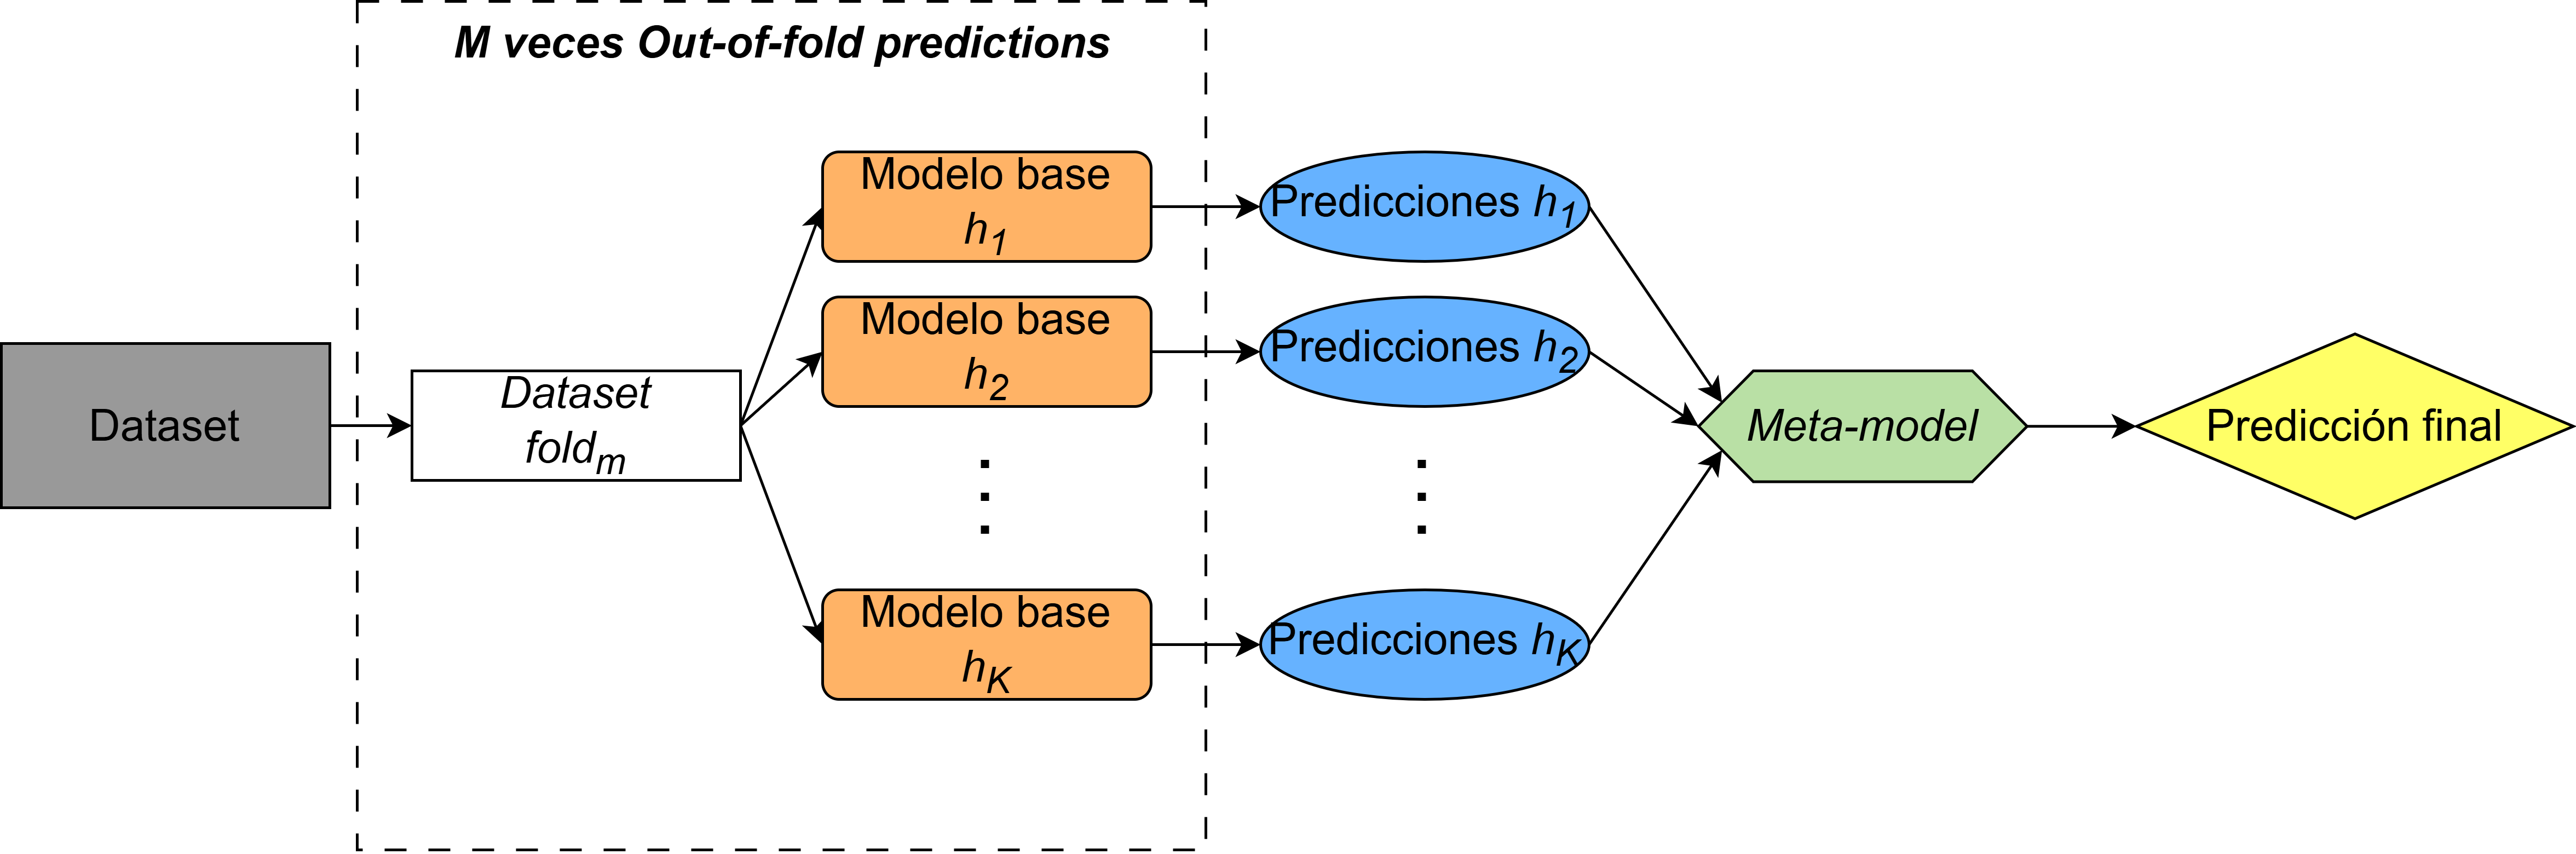
\includegraphics[width=\linewidth]{StackingDiagram.png}
    \caption{Diagrama del funcionamiento del \textit{stacking}}
    \label{fig:EnsStackDiag}
\end{figure}

Todo el desarrollo de esta técnica de ensamble se ha extraído de \cite{wolpert1992stacked}. Sea $\mathcal{T}=\{(X_i,y_i)\}^n_{i=1}$ el conjunto de entrenamiento, donde $X_i \in \mathbb{R}^p$ es un vector de características y $y_i \in \mathbb{R}$ (regresión) o $y_i \in \mathcal{C}$ (clasificación) las variables respuesta. Sean $h_1,\ldots,h_K$ los modelos base que se van a utilizar en el ensamble.

Entonces, cada estimador $h_k$ se entrena de forma independiente sobre $\mathcal{T}$ y genera predicciones para cada $X_i$: $Z_{ik}=h_k(X_i)$. El resultado es un conjunto de datos $\mathcal{Z}=\{(Z_i,y_i)\}^n_{i=1}$, donde $Z_i=(h_1(X_i),\ldots,h_K(X_i))$ funcionará como un conjunto de predictores para el \textit{meta-model}. Finalmente, se entrena un \textit{meta-model} $H$ sobre $\mathcal{Z}$.

Ahora el modelo está preparado para generar una prediccion $y$ sobre una nueva muestra $X$:
\begin{equation*}
    y=H(h_1(X),\ldots,h_K(X))
\end{equation*}

Los modelos base realizan las predicciones del mismo conjunto para el que son entrenados. La idea original de \cite{wolpert1992stacked} fue utilizar \textit{out-of-fold predictions}, para evitar entrenar el \textit{meta-model} con predicciones sobreajustadas.

Se divide el conjunto $\mathcal{T}$ en $M$ particiones. Para cada partición $fold_m$, se entrenan los $K$ modelos base $h_k^{(-m)}$ sobre $\mathcal{T} \setminus fold_i$ y se predice sobre $fold_m$ ($h_k^{(-m)}$ indica que el modelo se entrenó sin usar el $fold_m$). Tras completar el proceso, se tienen predicciones no sesgadas de los $K$ \textit{base model} sobre las $n$ muestras. Son estas predicciones las utilizadas para construir $\mathcal{Z}$ y entrenar el \textit{meta-model}. Finalmente, los $K$ modelos base $h_k$ son entrenados sobre todo el conjunto de entrenamiento $\mathcal{T}$, y el modelo está preparado para obtener predicciones sobre nuevas muestras.

\section{\textit{Bagging}}
El \textit{Bagging} (abreviatura de \textit{Bootstrap Aggregating}) es un ensamble homogéneo, con esto queremos decir que los modelos base tienen una estructura común. El objetivo es reducir la varianza a través de la combinación de múltiples modelos base, que son entrenados sobre distintas muestras generadas mediante remuestreo con reemplazo (\textit{bootstrap}) del conjunto de entrenamiento original. La predicción final se obtiene agregando (\textit{aggregating}) las predicciones individuales de los modelos base.

Desarrollando como en \cite{breiman1996bagging}. Sea $\mathcal{T}=\{(X_i,y_i)\}^n_{i=1}$ el conjunto de entrenamiento, donde $X_i \in \mathbb{R}^p$ es un vector de características e $y_i \in \mathbb{R}$ (regresión) o $y_i \in \mathcal{C}$ (clasificación) las variables respuesta. A partir de $\mathcal{T}$ y mediante \textit{bootstrap} (remuestreo con reemplazo), se generan $B$ subconjuntos $\mathcal{T}^{(1)}, \ldots, \mathcal{T}^{(B)}$.

Se entrena un modelo base $h^{(b)}$ sobre cada subconjunto $\mathcal{T}^{(b)}$. La predicción final sobre una nueva muestra $X$ se obtiene por agregación de las predicciones individuales de cada modelo base: promedio para regresión (izquierda) y clase más frecuente para clasificación (derecha).

\begin{equation*}
H(X)=\frac{1}{B}\sum^B_{b=1}h^{(b)}(X) \hspace{2cm}    H(X)=\operatorname{mode} \left \{ h^{(1)}(X), \ldots, h^{(B)}(X) \right \}
\end{equation*}

\begin{figure}[h]
    \centering
    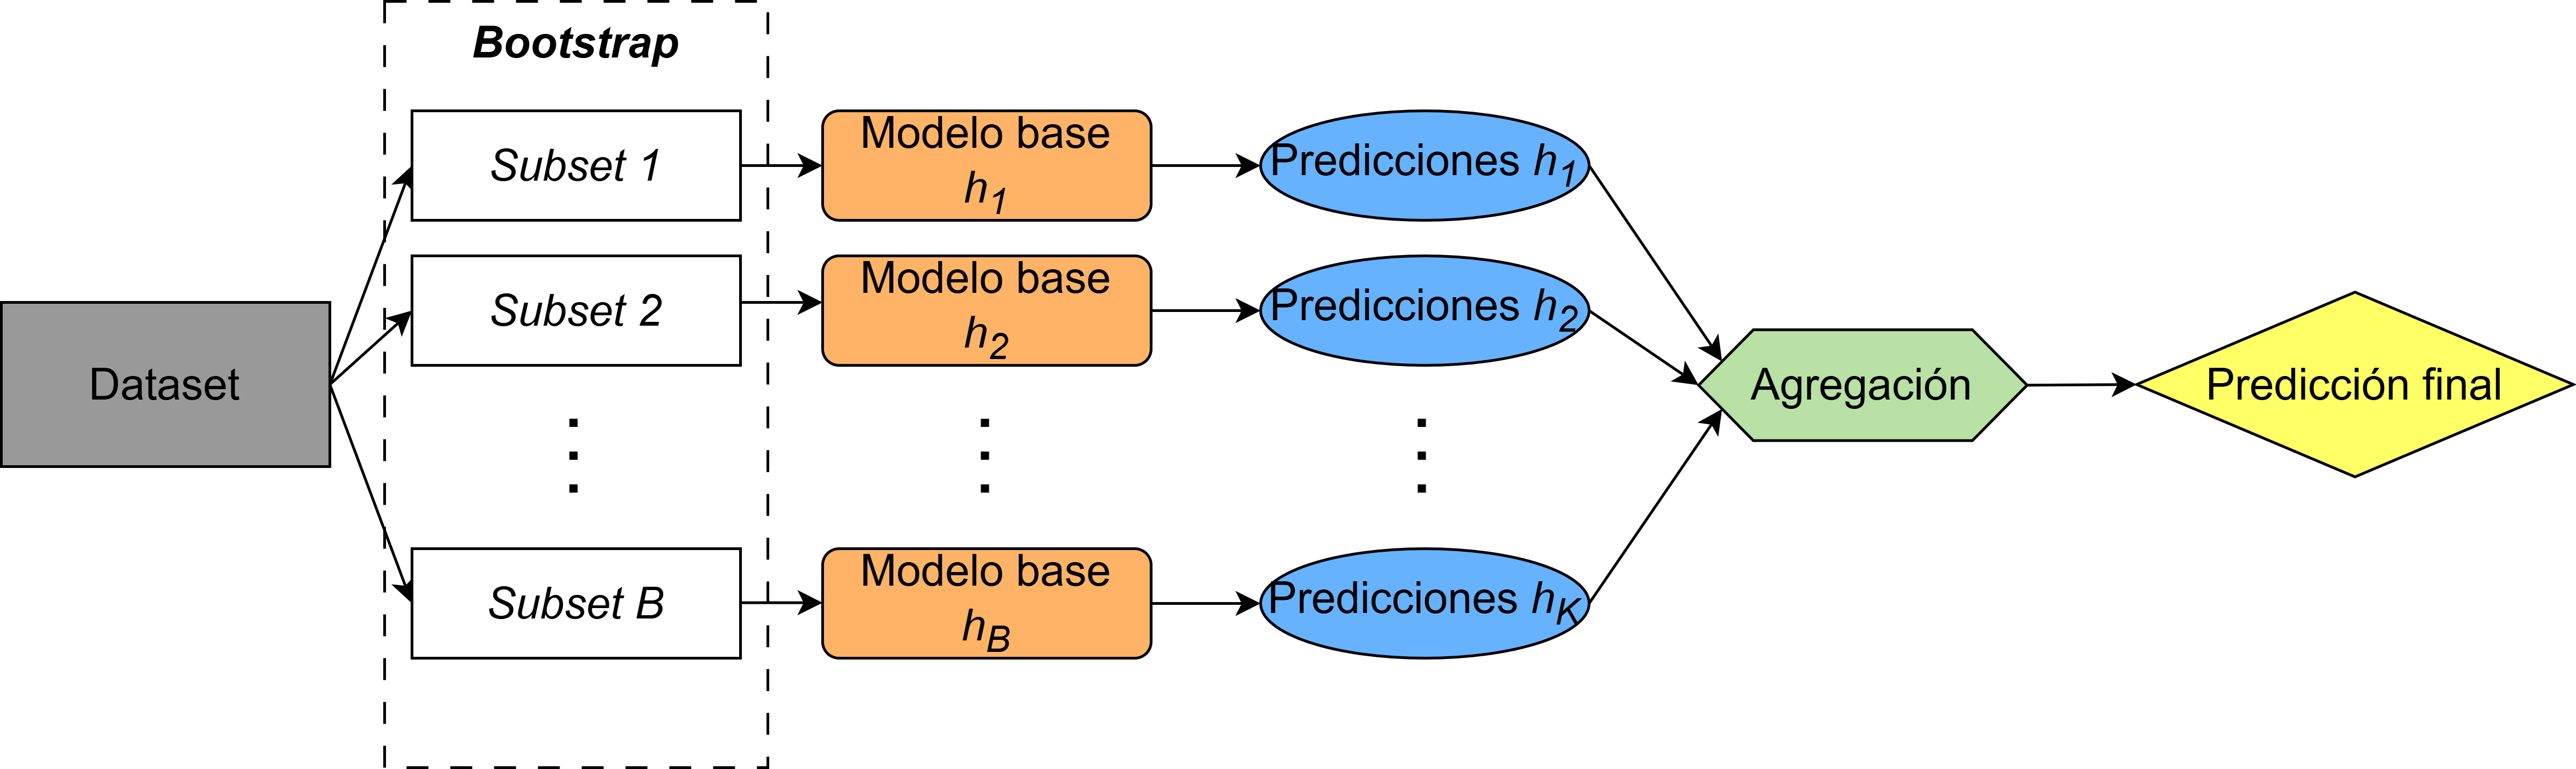
\includegraphics[width=\linewidth]{BaggingDiagram.png}
    \caption{Diagrama del funcionamiento del \textit{Bagging}}
    \label{fig:EnsBagDiag}
\end{figure}

Como se detalla en \cite{ISLP}, existe una forma muy directa de estimar el error de un modelo de \textit{bagging} sin tener que recurrir a \textit{k-fold cross-validation}. Cada modelo base $h^{(b)}$ es entrenado sobre un subconjunto generado por \textit{bootstrap} $\mathcal{T}^{(b)}$ del conjunto de entrenamiento original $\mathcal{T}$. En promedio, $\mathcal{T}^{(b)}$ contiene alrededor de $2/3$ de las observaciones en $\mathcal{T}$. Entonces, al conjunto $\mathcal{T} \setminus \mathcal{T}^{(b)}$ no utilizado durante el entrenamiento de $h^{(b)}$, que supone en torno a $1/3$ del conjunto de entrenamiento original, contiene las denominadas observaciones \textit{out-of-bag} (OOB).

Para obtener la predicción para una observación $(X_i,y_i)$ basta con utilizar aquellos modelos base $h^{(b)}$ cuyos subconjuntos de entrenamiento $\mathcal{T}^{(b)}$ no contengan dicha observación $(X_i,y_i)$ es decir, los modelos base para los que dicha observación es OOB. La prediccion OOB se obtiene por agregación de las predicciones de dichos modelos base para la $i-esima$ observación. Este proceso se repite para las $n$ observaciones y las predicciones OOB son utilizadas para computar el error.


\subsection{\textit{Random Forest}}
Como se detalla en \cite{ISLP} \textit{Random Forest} es un algoritmo considerado una extensión del \textit{bagging}. Conserva las características de este método de ensamble, utilizando como estimadores árboles de decisión, entrenándose cada uno con un subconjunto generado por \textit{bootstrap} del conjunto de entrenamiento original. Además, obtiene una estimación final agregando, como en cualquier otro \textit{bagging}, las predicciones de cada estimador.

La característica novedosa de este algoritmo es la implementación de un mecanismo explícito para reducir la correlación entre los múltiples árboles de decisión que componen el <<bosque>>. Y es que para la división de cada nodo, solo se tendrá en cuenta un subconjunto aleatorio del total de características. Esta introducción de aleatoriedad adicional induce a los árboles a explorar nuevas estructuras de decisión. Se permite que los árboles adquieran profundidad y no se aplican procesos de poda, por lo que, de forma individual, cada árbol, presentará un sesgo bajo pero una varianza alta. Tras agregar todos los árboles, el modelo final presenta una menor varianza, generalizando mejor a nuevos datos.

Como lo encontramos en \cite{breiman2001random}. Sea $\mathcal{P}= \{1,\ldots,p \}$ el conjunto de índices de las características. Recordando lo tratado en el apartado \ref{subsec:RecBinSplit}, una posible división venía dada por $\theta =(j,t_m)$, donde $j \in \mathcal{P}$, y $t_m$ es el valor umbral establecido para la división. Durante el proceso de \textit{recursive binary splitting} tratado en \ref{subsec:RecBinSplit}, \textit{Random Forest} introduce que para cada nodo se toma un subconjunto $\mathcal{F} \subset \mathcal{P}$ con $|\mathcal{J}|=k$ para evaluar la mejor división. De esta forma, cada posible división $\theta =(j,t_m)$ la característica se toma de este subconjunto $j \in \mathcal{F}$ y no del total de características.

\section{\textit{Boosting}}
Demostrada su viabilidad teóricamente en \cite{schapire1990strength}, \textit{boosting} es un método de ensamble que suele implementarse de forma homogénea. La diferencia sustancial con el \textit{bagging} es que los modelos base no son independientes, sino que se construyen de forma secuencial y aditiva: cada nuevo modelo se entrena prestando mayor atención a las observaciones que han sido mal predichas por sus predecesores. El modelo final es una combinación ponderada de los modelos débiles, en la que los mejores modelos tienen más influencia. Este ensamble final logra, en general, reducir el sesgo.

La atención a las observaciones que presentan mayor error en las predicciones de los modelos anteriores se logra mediante la asignación de pesos, que se ajustan iterativamente para favorecer la corrección de los casos más difíciles.

\begin{figure}[h]
    \centering
    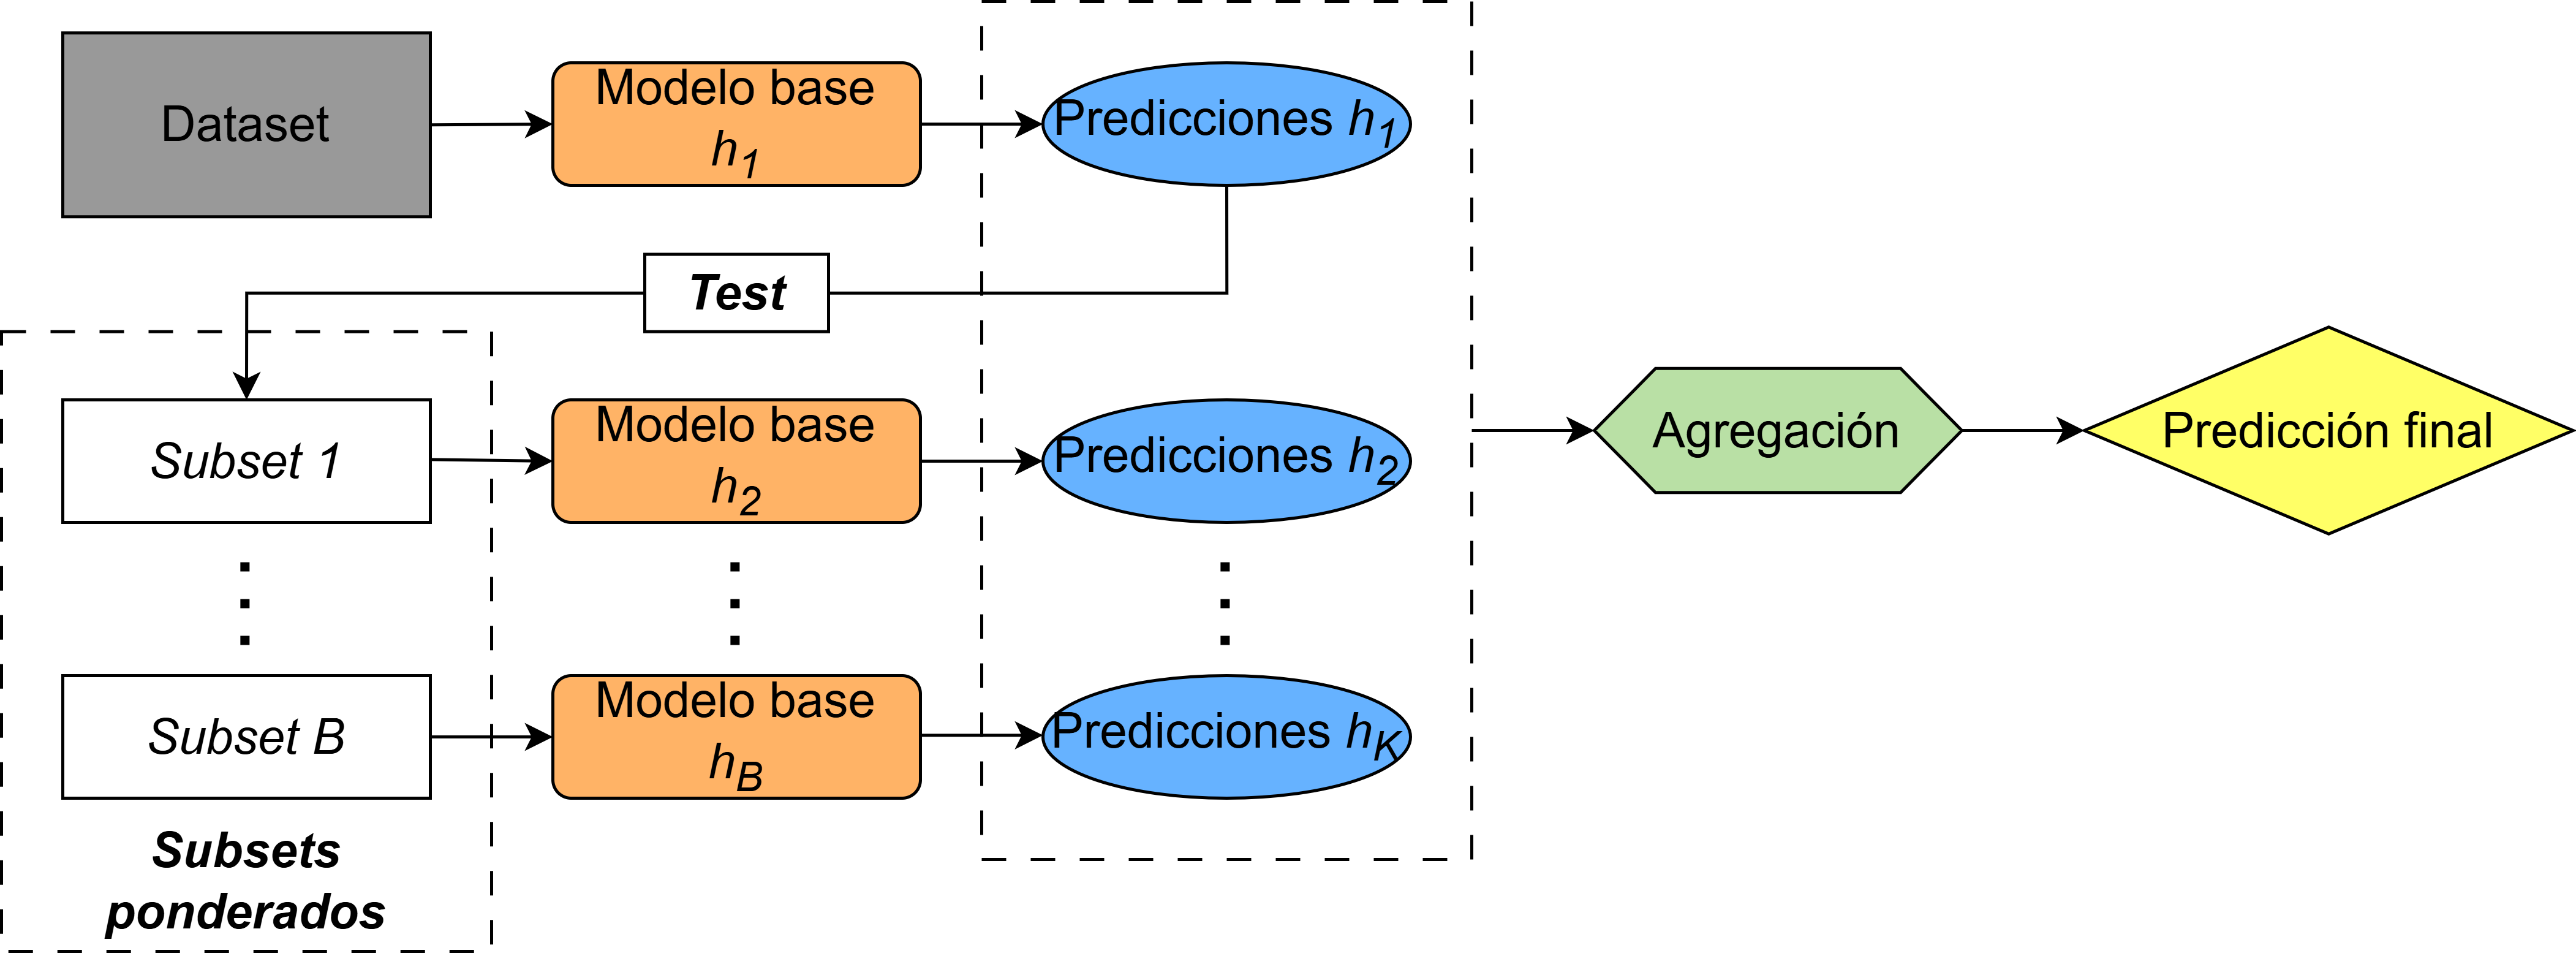
\includegraphics[width=\linewidth]{BoostingDiagram.png}
    \caption{Diagrama del funcionamiento del \textit{Boosting}}
    \label{fig:EnsBoostDiag}
\end{figure}

Existen múltiples algoritmos basados en esta metodología, como \textit{AdaBoost}, \textit{Gradient Boosting} o implementaciones modernas, como \textit{XGBoost}, que difieren en la forma en que calculan el error de los modelos base, actualizan los pesos de las muestras o combinan finalmente los modelos.


\subsection{\textit{AdaBoost}}
Introducido en \cite{freund1997decision}, se trata del algoritmo pionero en aplicar esta estrategia de ensamble. Originalmente concebido para clasificación binaria, se utilizan, en general, \textit{stumps} como modelos débiles, es decir, árboles de decisión de un solo nivel para conformar un clasificador binario fuerte.

Sea $\mathcal{T}=\{(X_i,y_i)\}^n_{i=1}$ el conjunto de entrenamiento, donde $X_i \in \mathbb{R}^p$ es un vector de características e $y_i \in \{-1,+1\}$ la variable de salida. Inicialmente, se asignan a las muestras $\{(X_i,y_i)\}^n_{i=1}$ pesos iguales:
\begin{equation*}
    w_i^{(1)}=\frac{1}{n}   \hspace{2cm}    \forall i=1,\ldots,n
\end{equation*}

Para cada iteración $t=1,\ldots,T$:
\begin{itemize}
    \item Se entrena un clasificador débil $h_t(X)$ utilizando los pesos correspondientes $\{w_i^{(t)}\}^n_{i=1}$. En particular, cuando se utilizan \textit{stumps} como modelos base, los pesos alteran el proceso de \textit{recursive binary splitting}, ponderando sobre estos pesos y priorizando la correcta clasificación de las muestras con mayor peso.

    \item Se calcula el error ponderado:\footnote{$\sum^n_{i=1}w_i^{(t)}=1$ $\forall t$ pues los pesos se normalizan tras cada actualización.}
        \begin{equation*}
            \varepsilon_t=\frac{\sum^n_{i=1}w_i^{(t)}\,1\{h_t(x_i) \neq y_i\}}{\sum^n_{i=1}w_i^{(t)}}
        \end{equation*}

    \item Se asigna un peso al clasificador:
        \begin{equation*}
            \alpha_t=\frac{1}{2}\,\ln \left( \frac{1-\varepsilon_t}{\varepsilon_t} \right)
        \end{equation*}
        que refleja su capacidad predictiva, cuanto menor es el error $\varepsilon_t$, mayor es el peso y, mayor será su influencia en el clasificador final.

    \item Se actualizan los pesos de las muestras:\footnote{Notar que los valores de $y_i,h_t(X_i) \in \{\pm 1 \}$.}
        \begin{equation*}
            w_i^{(t+1)}=w_i^{(t)}\exp \left( -\alpha_t\,y_i\,h_t(X_i)\right)
        \end{equation*}
        de forma que $ w_i^{(t+1)}=w_i^{(t)}\exp \left( -\alpha_t \right)$ para muestras bien clasificadas, mientras que $ w_i^{(t+1)}=w_i^{(t)}\exp \left( \alpha_t \right)$ cuando una muestra se clasifica erróneamente. Finalmente, se normalizan de forma que $\sum_{i=1}^n w_i^{(t+1)} = 1$.
\end{itemize}

El clasificador final $H(X)$ se obtiene como combinación lineal de los clasificadores débiles ponderados por sus pesos:
\begin{equation*}
    H(X)=sign \left( \sum_{t=1}^T \alpha_t h_t(X) \right)
\end{equation*}

De esta forma, el algoritmo \textit{AdaBoost} consigue, en general, reducir el sesgo iterativamente, al enfocarse progresivamente en las muestras más difíciles de clasificar en cada iteración.

Más adelante se introdujeron extensiones del algoritmo tanto para clasificación multiclase, como para regresión.

\subsection{\textit{Gradient Boosting}}
Formalmente descrito en \cite{friedman2001greedy}, \textit{Gradient Boosting} es un método de ensamble basado en el mismo principio que \textit{AdaBoost}. No obstante, a diferencia de este último, que actualiza los pesos de las muestras en cada iteración, la estrategia de \textit{Gradient Boosting} es plantear el proceso como un descenso de gradiente sobre una función de pérdida.

Sea $\mathcal{T}=\{(X_i,y_i)\}^n_{i=1}$ el conjunto de entrenamiento, donde $X_i \in \mathbb{R}^p$ es un vector de características e $y_i \in \mathbb{R}$ (regresión) ó $y_i \in \mathcal{C}$ (clasificación) las variables respuesta. Inicialmente, se define un modelo constante:

\begin{equation*}
    H_0(X)=\arg\min_{c}\sum^n_{i=1}\mathcal{L}(y_i,c)
\end{equation*}


En cada iteración $t=1, \ldots, T$:
\begin{itemize}
    \item Se calcula el gradiente negativo de la función de pérdida para cada muestra, lo que denominamos \textbf{pseudorresiduos}:
        \begin{equation*}
            r_{it}=-\left[ \frac{\partial \mathcal{L}(y,H(X_i))}{\partial H(X_i)} \right]_{H(X_i)=H_{t-1}(X_i)} \hspace{3cm}    i=1,\ldots,n
        \end{equation*}
        notar que como $H(X_i)$ utilizamos el modelo ensamblado hasta la iteración anterior $t-1$.

    \item Se entrena un nuevo modelo débil $h_t(X)$, generalmente un árbol de decisión poco profundo, utilizando como variables objetivo los pseudoresiduos calculados previamente. Es decir, en cada iteración utilizamos el conjunto de entrenamiento $\mathcal{T}^{(t)}={(X_i, r_{it})}_{i=1}^n$.

    \item Se calcula el coeficiente $\gamma_t$ óptimo que minimiza la función de pérdida. Este coeficiente determina la escala en que contribuye la dirección de descenso de gradiente estimada por $h_t$.
        \begin{equation*}
            \gamma_t=\arg\min_\gamma\sum_i\mathcal{L}(y_i,H_{t-1}(X_i)+\gamma h_t(X_i))
        \end{equation*}

    \item Se actualiza el modelo ensamblado con una tasa de aprendizaje $\nu \in (0,1]$, que es un hiperparámetro fijo que se escoge para todo el proceso de ensamble.
        \begin{equation*}
            H_t(X)=H_{t-1}(X)+\nu \gamma_t h_t(X)
        \end{equation*}
\end{itemize}.

Este proceso se repite hasta que se alcanza un criterio de parada, normalmente que la reducción de la pérdida sea mínima, o que el error en validación deje de reducirse.

\subsection{\textit{XGBoost}}
\textit{Extreme Gradient Boosting}, ampliamente conocido por su acrónimo \textit{XGBoost}, es un algoritmo de código abierto planteado como una extensión de \textit{Gradient Boosting}, en la que se implementan mejoras de rendimiento y optimización. Fue introducido formalmente en \cite{chen2016xgboost}, donde se detallan los principales aportes de este algoritmo. El proyecto mantiene una implementación activa que podemos consultar en \textit{GitHub}\footnote{https://github.com/dmlc/xgboost}.

Aunque a nivel práctico amplía el concepto de \textit{Gradient Boosting}, este algoritmo plantea un cambio estructural que afecta a la forma en que se construyen los árboles, por ello es conveniente introducir el concepto de \textit{Extreme Gradient Boosted Tree (XGBTree)}.

\subsubsection{XGBTree}
Por cuestión de claridad, realizamos un cambio de notación y el árbol de decisión entrenado en la iteración $t$ vendrá dado por $f_t$. Además, su predicción para la muestra $i$ vendrá dada por $\hat{y}^{(t)}_i$:

\begin{equation*}
    \begin{aligned}
        \hat{y}^{(1)}_i &=   f_1(X_i)\\
        \hat{y}^{(2)}_i &=  f_1(X_i)+f_2(X_i)   =   \hat{y}^{(1)}_i+f_2(X_i)\\
        &\,\,\,\vdots\\
        \hat{y}^{(t)}_i &=  \sum_{t}f_t(X_i)=   \hat{y}^{(t-1)}_i+f_t(X_i)\\
    \end{aligned}
\end{equation*}

El cambio fundamental a la hora de entrenar estos árboles es que a la hora de construirse, no nos limitamos a elegir como variable objetivo unos pseduorresiduos, sino que se introduce el descenso del gradiente en la misma función de pérdida que usamos para evaluar cada división del árbol. Además, se añade un término de regularización $\Omega(f_t)$ que controla la complejidad y el número de hojas del árbol. Para una iteración $t$, evaluamos la que vamos a denominar \textbf{función objetivo} $\mathcal{L}^{(t)}$, que tendrá que minimizarse durante el entrenamiento del árbol:

\begin{equation*}
    \mathcal{L}^{(t)}=\sum_{i=1}^n\ell(y_i,\hat{y}^{(t-1)}_i+f_t(X_i))+\Omega(f_t)
\end{equation*}
donde $\ell$ es la función de pérdida empírica (error cuadratico, log-loss, ...).

Ahora, podemos tomar la expansión de Taylor hasta segundo orden de la función de pérdida:

\begin{equation*}
    \mathcal{L}^{(t)}=\sum_{i=1}^n \left[ \ell(y_i,\hat{y}_i^{(t-1)})+g_if_t(X_i)+\frac{1}{2}h_i f_t(X_i)^2 \right] + \Omega(f_t)
\end{equation*}
donde como primera y segunda derivada de la función de pérdida están relacionadas con gradiente y hessiano, se utiliza la notación $g_i$ y $h_i$, que se definen:

\begin{equation*}
    g_i=:\frac{\partial \ell(y_i,\hat{y}_i^{(t-1)})}{\partial \hat{y}_i^{(t-1)}} \hspace{2cm} h_i=:\frac{\partial \ell(y_i,\hat{y}_i^{(t-1)})}{\partial^2 \hat{y}_i^{(t-1)}}
\end{equation*}

Tras eliminar las constantes, la función objetivo resulta:

\begin{equation*}
    \mathcal{L}^{(t)}=\sum_{i=1}^n \left[g_if_t(X_i)+\frac{1}{2}h_i f_t(X_i)^2 \right] + \Omega(f_t)
\end{equation*}
donde $g_i$ y $h_i$ dependen de la predicción anterior, mientras que $f_t(X_i)$ hace referencia a la predicción del árbol que estamos construyendo. Podemos interpretar este entrenamiento como un árbol que no solo sigue la dirección del gradiente, sino que también tiene en cuenta la curvatura de la función de pérdida, con lo que se consigue mejor precisión.

La función objetivo cuenta además con un término de regularización $\Omega(h_t)$. En primer lugar, redefinimos el árbol $f_t$:

\begin{equation*}
    f_t(X_i)=w_{q(X_i)}, w\in R^J, q:R^n\rightarrow R^J
\end{equation*}
donde $w$ es un vector con las predicciones correspondientes a cada hoja del árbol $f_t$ y $q$ una función que asigna a cada muestra $X_i$ una hoja del árbol, con $J$ el número total de hojas. Definimos el término de regularización como:

\begin{equation*}
    \Omega(f_t)=\gamma J + \frac{1}{2} \lambda \sum_{j=1}^J w_j^2
\end{equation*}
donde el término $\gamma J$ penaliza el número de hojas, favoreciendo árboles más sencillos y evitando divisiones que no tengan aportes significativos en la reducción de perdida, mientras que el término $\frac{1}{2} \lambda \sum_{j=1}^J w_j^2$ limita la magnitud de la predicción de las hojas, impidiendo pasos demasiado grandes en la dirección del gradiente.

Con esta reformulación, podemos reescribir la función objetivo para el $t-esimo$ árbol como:

\begin{equation*}
    \begin{aligned}
        \mathcal{L}^{(t)} =& \sum_{i=1}^n \left[g_i w_{q(X_i)}+\frac{1}{2}h_i w_{q(X_i)}^2 \right] + \gamma J + \frac{1}{2} \lambda \sum_{j=1}^J w_j^2\\ =& \sum_{j=1}^J \left[ \left( \sum_{i\in Q_j} g_i \right) w_j+\frac{1}{2} \left( \sum_{i\in Q_j} h_i+\lambda \right) w_j^2 \right] + \gamma J
    \end{aligned}
\end{equation*}
donde $Q_j$ es el conjunto de muestras en la hoja $j$, es decir, $i \in Q_j$ son las muestras en la hoja $j$. Notar entonces que hemos cambiado el índice del sumatorio, pues todas las muestras de la hoja $j$ obtienen la misma predicción. Podemos ahora compactar la expresión definiendo $G_j=\sum_{i \in Q_j}g_i$ y $H_j=\sum_{i \in Q_j}h_i$:

\begin{equation*}
     \mathcal{L}^{(t)} = \sum_{j=1}^J \left[ G_j w_j+\frac{1}{2} H_j w_j^2 \right] + \gamma J
\end{equation*}

Como las $w_j$ son independientes, para una estructura de árbol $q(X_i)$ dada, podemos obtener analíticamente la reducción óptima de la función objetivo:

\begin{equation*}
    \begin{aligned}
        w_j^*=&-\frac{G_j}{H_j+\lambda}\\
        \mathcal{L}^{(t)*}=&-\frac{1}{2}\sum_{j=1}^T\frac{G_j^2}{H_j+\lambda}+\gamma J
    \end{aligned}
\end{equation*}
$\mathcal{L}^{(t)*}$ nos sirve como una suerte de puntuación de que tan buena es una estructura de árbol $q(X_i)$.

Con esto ya tenemos un marco para medir la calidad de un árbol. Idealmente, generaríamos todos los posibles árboles y nos quedaríamos con el mejor. No obstante, en la práctica esto es inviable, por lo que recurrimos a estrategias de optimización para cada división. Definimos la ganancia de una división como:

\begin{equation*}
        Gain=\frac{1}{2}\left[  \underbrace{\frac{G_L^2}{H_L+\lambda}}_{(1)}+\underbrace{\frac{G_R^2}{H_R+\lambda}}_{(2)}-\underbrace{\frac{(G_L+G_R)^2}{H_L+H_R+\lambda}}_{(3)}\right] - \underbrace{\gamma}_{(4)}
\end{equation*}
donde el término $(1)$ es la puntuación de la hoja izquierda, $(2)$ es la puntuación de la hoja derecha y $(3)$ es la puntuación de la hoja original. $(4)$ es el término de regularización correspondiente a la adición de una nueva hoja: si la ganancia es menor que $\gamma$, no se añadirá esa rama (se comporta como un término de poda).

Sea $\mathcal{T}=\{(X_i,y_i)\}^n_{i=1}$ el conjunto de entrenamiento, donde $X_i \in \mathbb{R}^p$ es un vector de características e $y_i \in \mathbb{R}$ (regresión) ó $y_i \in \mathcal{C}$ (clasificación) las variables respuesta. Inicialmente, se define un modelo constante:

\begin{equation*}
    F_0(X)=\arg\min_{c}\sum^n_{i=1}\mathcal{L}(y_i,c)
\end{equation*}


En cada iteración $t=1, \ldots, T$:
\begin{itemize}
    \item Se computan los gradientes $g_i$ y hessianas $h_i$ correspondientes a todas las muestras:\footnote{Recordemos que $\hat{y}_i^{(t-1)}$ corresponde con la predicción $f_{t-1}(X_i)$.}
    \begin{equation*}
        g_i=:\frac{\partial \ell(y_i,\hat{y}_i^{(t-1)})}{\partial \hat{y}_i^{(t-1)}} \hspace{2cm} h_i=:\frac{\partial \ell(y_i,\hat{y}_i^{(t-1)})}{\partial^2 \hat{y}_i^{(t-1)}}
    \end{equation*}

    \item Se entena el árbol $f_t$ utilizando los $g_i$ y $h_i$ para calcular la ganancia de cada división.

    \item Se actualiza el modelo ensamblado utilizando la tasa de aprendizaje $\eta \in (0,1]$: 
    \begin{equation*}
        F_t(X)=F_{t-1}(X)+\eta f_t
    \end{equation*}
\end{itemize}

Finalmente, el modelo ensamblado final es $F_T(X)=F_0(X)+\eta \sum_{t=1}^P f_t$.


\chapter[Estimacion de $T_c$]{Estimación de la temperatura crítica de superconductores}
\section{Introducción}
La resistividad eléctrica de un conductor metálico disminuye gradualmente cuando la temperatura se reduce. En conductores ordinarios, se alcanza un valor límite, de modo que mantienen una resistencia no nula incluso cerca del cero absoluto. La resistencia de un superconductor, en cambio, desciende bruscamente a cero cuando el material se enfría por debajo de su temperatura crítica ($T_c$).

En 1911, el físico neerlandés Heike Kamerlingh Onnes observó que la resistencia eléctrica del mercurio desaparecía bruscamente al enfriarse a 4K. Este hallazgo, junto con el desarrollo de las técnicas necesarias para licuar helio y alcanzar dichas temperaturas, le valieron el premio Nobel de Física. Al tratarse la superconductividad de un fenómeno esencialmente cuántico, tuvieron que pasar varias décadas hasta que se produjeron los primeros avances en la comprensión de este fenómeno: las teorías BCS y de Ginzburg-Landau.

Tras algunos años sin avances significativos, se descubrió una familia de materiales cerámicos, los óxidos de cobre con estructura de perovskita, que eran superconductores con temperaturas críticas superiores a 90K. Estos materiales, conocidos como superconductores de alta temperatura, abrieron la puerta a aplicaciones tecnológicas viables, al mantener la superconductividad en condiciones más accesibles.

Entre sus aplicaciones más destacadas se encuentran los equipos de resonancia magnética nuclear utilizados en hospitales, los sistemas de transporte por levitación magnética y, en el ámbito científico, el direccionamiento de haces en aceleradores de partículas o la fabricación de qubits para computadores cuánticos.

No obstante, la predicción teórica de la temperatura crítica de un superconductor continúa siendo un problema abierto más de un siglo después de su descubrimiento. Ante la ausencia de modelos predictivos basados en la teoría, la experimentación empírica ha guiado históricamente la síntesis de nuevos materiales superconductores. En este contexto, el aprendizaje automático (Machine Learning) se perfila como una herramienta prometedora para abordar este desafío. En este estudio, utilizaremos algunas de las técnicas explicadas con anterioridad con el objetivo de estimar la temperatura crítica ($T_c$) de superconductores a partir de sus propiedades físicas y químicas, extraídas directamente de su fórmula química.

Los datos empleados provienen originalmente de la base de datos de materiales superconductores mantenida por el Instituto Nacional para la Ciencia de Materiales (NIMS) de Japón. En particular, el conjunto de datos utilizado en este trabajo es el resultado de una cuidadosa minería y depuración de datos realizada sobre dicha base original, descrita detalladamente en \cite{hamidieh2018data}, de la que se han extraído una serie de descriptores físico-químicos interpretables por los algoritmos de aprendizaje automático.

\section{Conjuntos de datos y descriptores}
El conjunto de datos que vamos a utilizar cuenta con 81 características extraídas de 21.263 superconductores cuya temperatura crítica es conocida. Inicialmente, se tienen 8 propiedades referidas a los elementos que conforman los compuestos:

\begin{itemize}
\item \textbf{Masa atómica $[UMA]$}: masa atómica del elemento en reposo.
\item \textbf{Primera energía de ionización \textit{(fie)} $[kJ/mol]$}: energía requerida para quitar de un átomo un electrón de valencia
\item \textbf{Radio atómico $[pm]$}: radio del átomo del elemento.
\item \textbf{Densidad $[kg/m^3]$}: densidad del elemento en condiciones estándar de presion y temperatura.
\item \textbf{Afinidad electrónica $[kJ/mol]$}: energía requerida para añadir un electrón a un átomo neutro.
\item \textbf{Calor de fusión $[kJ/mol]$}: energía necesaria para cambiar de fase só0lida a líquida el elemento sin cambio de temperatura (calor latente de fusión).
\item \textbf{Conductividad térmica $[W/(m \cdot K)]$}: coeficiente $(\kappa)$ de conductividad térmica del elemento.
\item \textbf{Valencia}: número típico de enlaces que forma el elemento.
\end{itemize}

Con estas propiedades elementales se generan 10 familias de descriptores estadísticos referentes a los compuestos:
\begin{multicols}{2}
\begin{itemize}
    \item \textbf{mean\_*} $=\mu = \frac{1}{n} \sum_{i=1}^{n} t_i$
    \item \textbf{wtd\_mean\_*} $=\nu = \sum_{i=1}^{n} w_i t_i$
    \item \textbf{gmean\_*} $=\left(\prod_{i=1}^{n} t_i\right)^{1/n}$
    \item \textbf{wtd\_gmean\_*} $=\left(\prod_{i=1}^{n} t_i^{w_i}\right)^{1/n}$
    \item \textbf{entropy\_*} $=-\sum_{i=1}^{n} p_i \log(p_i)$
    \item \textbf{wtd\_entropy\_*} $=-\sum_{i=1}^{n} \frac{w_i\, p_i}{\sum_{j=1}^{n} w_j\, p_j} \log{\left(\frac{w_i\, p_i}{\sum_{j=1}^{n} w_j\, p_j}\right)}$
    \item \textbf{range\_*} $=\max_i(t_i)-\min_i(t_i)$
    \item \textbf{wtd\_range\_*} $=\max_i(w_i t_i)-\min_i(w_i t_i)$
    \item \textbf{std\_*} $=\sqrt{\frac{1}{n}\sum_{i=1}^{n}(t_i-\mu)^2}$
    \item \textbf{wtd\_std\_*} $=\sqrt{\sum_{i=1}^{n} w_i (t_i-\nu)^2}$
\end{itemize}
\end{multicols}
donde $n$ es el número de átomos que conforman el compuesto, $t_i$ es el valor de la propiedad para el elemento $i$, $w_i$ corresponde con la estequeometría normalizada del elemento $i$, y $p_i=\frac{t_i}{\sum_{j=1}^{n} t_j}$.

El resultado son 10 familias de descriptores estadísticos, cada una de las cuales está formada por 8 características (una por cada propiedad elemental). Se añade además una nueva propiedad:
\begin{itemize}
    \item \textbf{Número de elementos \textit{(number\_of\_elements)}}: número de elementos químicos distintos presentes en la fórmula del compuesto.
\end{itemize}

Antes de proceder a la construcción de los modelos predictivos, es fundamental realizar un análisis exploratorio de los datos con el objetivo de comprender con mayor profundidad la estructura del conjunto de datos, evaluar la distribución de las variables y detectar patrones relevantes. En el apéndice \ref{ap:EDA} se detalla el estudio llevado a cabo.

\section{Modelado}
Para el modelado se ha decidido inicialmente utilizar \textit{Random Forest} y \textit{XGBoost}, ambos basados en el principio de ensamblado de árboles de decisión. No obstante, se incluye en el estudio un árbol de decisión simple con el objetivo de cuantificar la mejora de rendimiento que proporcionan las técnicas de ensamble.

Tanto el árbol de decisión simple como los modelos base que componen el \textit{Random Forest} emplean el error cuadrático medio (MSE) como criterio de partición durante el entrenamiento. De forma análoga, \textit{XGBoost} optimiza originalmente MSE en su proceso de descenso del gradiente de segundo orden. Todo el código implementado para realizar el estudio puede encontrarse en el repositorio de \textit{GitHub} \cite{barba_tfg_repo}.

\subsection{Métricas de evaluación}
Antes de sumergirnos en el entrenamiento de los modelos, es importante establecer cuáles serán las métricas de evaluación utilizadas para cuantificar su desempeño. Tradicionalmente en problemas de regresión, se han utilizado la raíz cuadrada del error cuadrático medio $(RMSE)$ y el coeficiente de determinación $(R^2)$:

\begin{equation*}
    RMSE=\sqrt{\sum_{i=1}^n \frac{(\hat{y}_i-y_i)^2}{n}} \hspace{3cm}  R^2=1-\frac{\sum_{i=1}^n (y_i-\hat{y}_i)^2}{\sum_{i=1}^n (y_i-\bar{y}_i)^2}
\end{equation*}

El $RMSE$ proporciona información de la desviación promedio entre los valores predichos por el modelo y los observados experimentalmente. Por su parte, $R^2$ indica la proporción de la variabilidad de resultados que es explicada por el modelo, por ello, sirve como una medida de la calidad del ajuste.

Se contempla también el uso de una métrica más. El error porcentual absoluto medio $(MAPE)$ nos aportará también una medida de la precisión relativa de las estimaciones:

\begin{equation*}
    MAPE=\frac{100}{n} \sum_{i=1}^n \left|\frac{\hat{y}_i-y_i}{y_i}\right|
\end{equation*}

El $MAPE$ se calcula como el promedio del error porcentual absoluto con respecto al valor experimental real. Es importante tener en cuenta que nuestra variable objetivo abarca varios órdenes de magnitud, con valores que van desde $0.00021\,K$, hasta $185\,K$. Al evaluar nuestros resultados mediante el $MAPE$, los errores absolutos pequeños, dado el rango de valores que puede tomar la temperatura crítica, provocarán que, para las muestras en la región de temperaturas bajas, esta métrica crezca de forma descontrolada.

Por esta razón, se decide utilizar el error porcentual absoluto medio simétrico $sMAPE$, que corrige este sesgo al normalizar el error con respecto a la media entre el valor real y el estimado, proporcionándonos una medida más equilibrada.

\begin{equation*}
    sMAPE=\frac{100}{n} \sum_{i=1}^n \left|\frac{\hat{y}_i-y_i}{(\hat{y}_i+y_i)/2}\right|
\end{equation*}


\subsection{Evaluación previa}
Antes de comenzar el entrenamiento de los modelos, se realiza la partición de los datos en dos subconjuntos: uno destinado a entrenamiento y otro a la validación, que permitirán evaluar correctamente el rendimiento de los modelos.

Con el objetivo de seleccionar los algoritmos con mejor desempeño antes del ajuste final, se procede con una evaluación preliminar mediante validación cruzada sobre el conjunto de entrenamiento. En la Tabla \ref{tab:prev_crossval} se pueden ver los resultados obtenidos.

\begin{table}[H]
    \centering
    \caption{Métricas de evaluación obtenidas para la validación cruzada sobre el conjunto de entrenamiento.}
    \begin{tabular}{r|c|c|c}
                               & \textbf{$RMSE$} & \textbf{$R^2$} & \textbf{$sMAPE$} \\ \hline
        \textbf{Random Forest} & 9.718           & 0.920          & 26.373           \\ \hline
        \textbf{XGBoost}       & 9.787           & 0.919          & 32.424           \\ \hline
        \textbf{Decision Tree} & 12.403          & 0.869          & 29.186          
    \end{tabular}
    \label{tab:prev_crossval}
\end{table}

Como podemos ver reflejado en el $RMSE$, las predicciones del árbol de decisión simple son, en términos absolutos, de peor calidad que las obtenidas por los métodos de ensamble. No obstante, resulta llamativo el resultado obtenido por este modelo en la métrica $sMAPE$, pues logra superar al \textit{eXtreme Gradient Boosting}. La explicación reside en que el $sMAPE$ es menos sensible que el $RMSE$ a valores extremos y, puesto que los árboles de decisión simples tienden a generar predicciones más conservadoras y centradas, reducen los errores relativos porcentuales. A pesar de ello, este modelo no consigue explicar con la misma eficacia que los algoritmos de ensamble la variabilidad de la temperatura crítica, tal como refleja su $R^2$

Los resultados obtenidos por los modelos basados en técnicas de ensamble son, en cambio, bastante prometedores, considerando el rango de valores que puede adoptar la variable objetivo. Ambos alcanzan un coeficiente de determinación $R^2$ superior a $0.9$ y un $RMSE$ inferior a $9.8$. Por este motivo, se decide prescindir del árbol de decisión simple para las fases posteriores del estudio, centrando el análisis en los dos modelos con mayor potencial.

\section{Resultados}
Se procede ahora al entrenamiento de los modelos basados en métodos de ensamble sobre la totalidad del conjunto de entrenamiento, con el fin de evaluar su rendimiento de forma más representativa. En esta fase, la evaluación se da únicamente sobre el conjunto de validación, por lo que los resultados deben mostrar una ligera mejora respecto a los obtenidos durante la evaluación previa. Esto es debido a que, al emplearse un mayor volumen de datos durante el entrenamiento, mejora el ajuste de los modelos a las relaciones subyacentes. En la Tabla \ref{tab:res_train} podemos observar los resultados obtenidos.

\begin{table}[H]
    \centering
    \caption{Métricas de evaluación obtenidas para el entrenamiento general y calculadas sobre el conjunto de validación.}
    \begin{tabular}{r|c|c|c}
                               & \textbf{$RMSE$} & \textbf{$R^2$} & \textbf{$sMAPE$} \\ \hline
        \textbf{Random Forest} & 9.042           & 0.929          & 25.187           \\ \hline
        \textbf{XGBoost}       & 8.973           & 0.925          & 32.975
    \end{tabular}
    \label{tab:res_train}
\end{table}

Como podemos apreciar, ambos modelos presentan una mejora general respecto a la evaluación previa. Comprobamos una disminución del $RMSE$ y un incremento en $R^2$ en ambos algoritmos. \textit{Random Forest} logra un desempeño ligeramente mayor en términos de $sMAPE$. En conjunto, los resultados confirman que los métodos de ensamble ofrecen una capacidad predictiva sólida para este problema de regresión.

Sabemos que, escogiendo los hiperparámetros adecuados, es posible lograr una mejora en la capacidad predictiva de los modelos. Los algoritmos utilizados proporcionan herramientas que, por procesos heurísticos y a través de validación cruzada, son capaces de encontrar los hiperparámetros que optimizan el rendimiento del modelo. En la Tabla \ref{tab:res_tun} se pueden consultar los resultados obtenidos tras esta optimización.

\begin{table}[H]
    \centering
    \caption{Métricas de evaluación obtenidas tras el tuneo de hiperparámetros y calculadas sobre el conjunto de validación.}
    \begin{tabular}{r|c|c|c}
                               & \textbf{$RMSE$} & \textbf{$R^2$} & \textbf{$sMAPE$} \\ \hline
        \textbf{Random Forest} & 8.979           & 0.930          & 25.740           \\ \hline
        \textbf{XGBoost}       & 8.668           & 0.935          & 27.606
    \end{tabular}
    \label{tab:res_tun}
\end{table}

Tras el ajuste, ambos modelos mantienen un rendimiento estable, presentando una mejora ligera con respecto al entrenamiento inicial. El algoritmo \textit{XGBoost} alcanza los mejores resultados en términos de $R^2$ y $RMSE$, consolidándose como el de mayor capacidad explicativa global. Por su parte, el \textit{Random Forest} presenta un $sMAPE$ inferior, es decir, en términos relativos, sus predicciones son más estables.

En la Figura \ref{fig:res_PredReal} se muestran los gráficos comparativos entre los valores reales y predichos por cada modelo. De esta forma se puede analizar visualmente la dispersión de las predicciones en cada rango de temperaturas críticas.

\begin{figure}[h]
    \centering
    \includegraphics[width=0.85\textwidth]{real_Pred_1.png}
    \caption{Comparación entre valores reales y predichos. \textit{Random Forest} a la izquierda y \textit{XGBoost} a la derecha.}
    \label{fig:res_PredReal}
\end{figure}

Analizando brevemente la Figura \ref{fig:res_PredReal}, comprobamos cómo los puntos se concentran en torno a la diagonal, que precisamente correspondería con las predicciones perfectas. No obstante, podemos observar predicciones realmente alejadas de sus respectivos valores reales. La dispersión en la región de la diagonal, así como los valores mal predichos, explican que los resultados obtenidos para el $sMAPE$ superen el $25\%$.

Los modelos de ensamble basados en árboles son capaces de obtener una estimación de la importancia de cada variable en el proceso de predicción. En la Figura \ref{fig:res_impVar} se detallan las importancias calculadas por nuestros modelos. Esta medida se obtiene a partir del número de divisiones en las que participa un determinado descriptor en la totalidad de árboles que componen en ensamble. Dependiendo del método de ensamble, es una medida más o menos certera, esto se debe a que el diseño del algoritmo puede afectar a la proporcionalidad entre la frecuencia de uso de una variable y la relevancia real en la relación subyacente.

\begin{figure}[h]
    \centering
    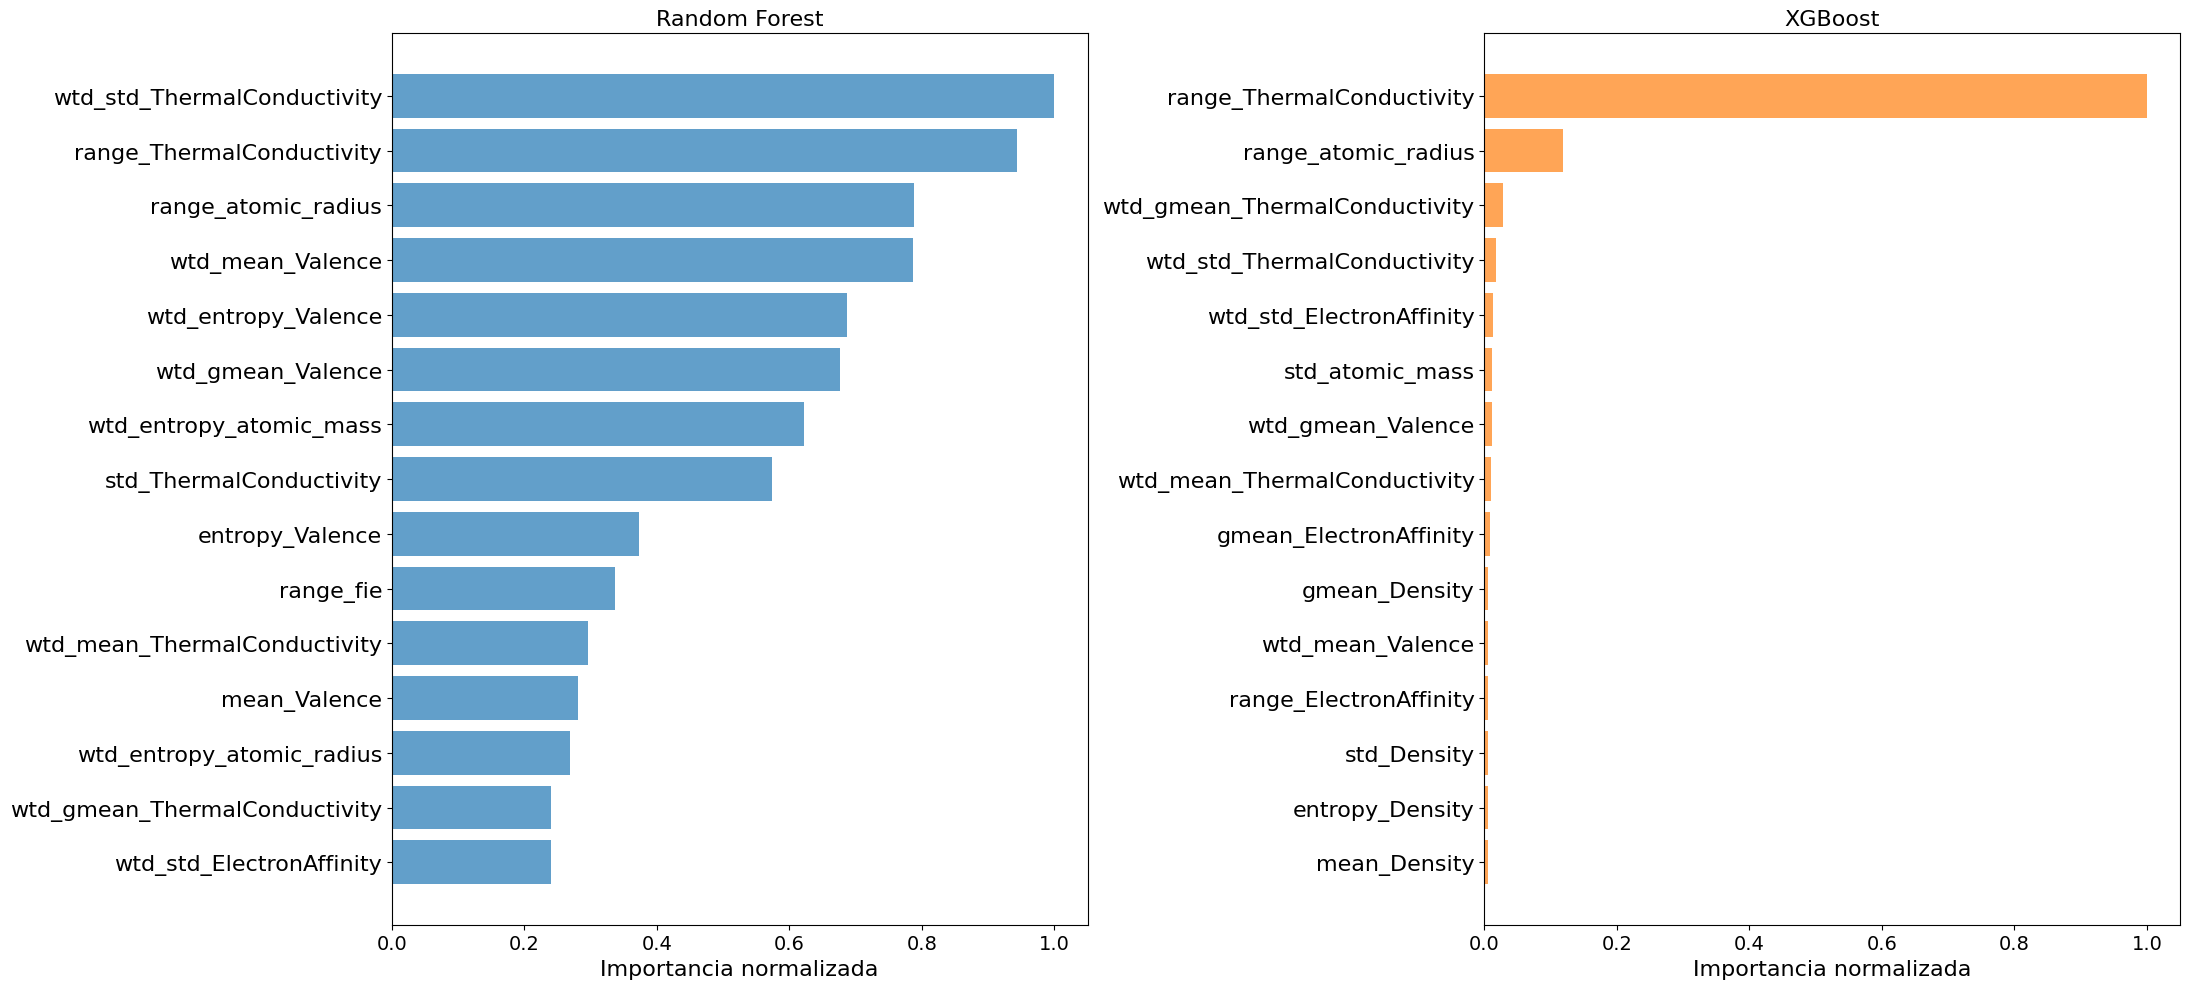
\includegraphics[width=0.85\textwidth]{impVar_1.png}
    \caption{Variables más relevantes para cada modelo. \textit{Random Forest} a la izquierda y \textit{XGBoost} a la derecha.}
    \label{fig:res_impVar}
\end{figure}

De la Figura \ref{fig:res_impVar} podemos extraer ciertas conclusiones: la conductividad térmica de los elementos que componen el material superconductor adquiere una gran relevancia. Particularmente, el rango entre los valores máximo y mínimo de esta propiedad se encuentra entre los descriptores con mayor peso en ambos modelos. Conviene ahora rescatar los resultados del análisis exploratorio de los datos \ref{ap:EDA}, en el que ya se había intuido la relevancia de este descriptor. El radio atómico de los elementos del compuesto y, en particular, su rango de variabilidad, también presenta una contribución significativa en la predicción de la temperatura crítica. Por último, cabe destacar las apariciones de la media ponderada de la valencia en \textit{Random Forest}, y de la desviación estándar ponderada de la afinidad electrónica en \textit{XGBoost}. Otras propiedades como la masa atómica o la primera energía de ionización (fie) tienen también una relevancia notoria.

Para el caso de \textit{XGBoost} se puede comprobar cómo el rango de variabilidad de la conductividad térmica concentra una proporción muy elevada de la importancia total. Este comportamiento puede atribuirse al mecanismo de aprendizaje de este método de ensamble, que focaliza la creación de nuevos árboles en las observaciones más difíciles de predecir. El resultado es que los descriptores más útiles para corregir los errores previos aparecen con mayor frecuencia, lo que finalmente se ve reflejado en la importancia relativa.

\section{Conclusiones}
Los resultados obtenidos demuestran la capacidad de estos modelos para capturar las tendencias globales del fenómeno estudiado, prueba de ello es un $RMSE$ inferior a $9$  y un $R^2$ por encima de $0.9$ en ambos modelos. Sin embargo, a nivel de predicción individual, su precisión resulta más limitada, tal como reflejan las métricas relativas como el $sMAPE$, la cual no ha podido reducirse por debajo del $25\%$.

Por otro lado, la interpretabilidad y la posibilidad de analizar la importancia de las variables constituyen una ventaja significativa en contextos de investigación científica, donde comprender las relaciones subyacentes es tan relevante como predecir con exactitud.

En conjunto, este proyecto nos permite comprender el funcionamiento de diversas herramientas de aprendizaje automático y su aplicación a un caso científico real. En este estudio se han expuesto las bases del \textit{Machine Learning}, los fundamentos matemáticos que sustentan los árboles de decisión y las principales técnicas de ensamble: \textit{stacking}, \textit{bagging} y \textit{boosting}. Para finalizar, hemos llevado dos de los algoritmos estudiados al terreno práctico.

En un panorama dominado por el auge de la inteligencia artificial moderna y los modelos de \textit{Deep Learning}, este trabajo pone en valor el potencial y la vigencia de los métodos basados en árboles de decisión. Aunque no siempre alcanzan el rendimiento de las redes neuronales en grandes volúmenes de datos, su equilibrio entre precisión, robustez y explicabilidad los convierten en herramientas especialmente adecuadas para problemas científicos con conjuntos de datos acotados y alta necesidad de interpretabilidad.


\printbibliography

\appendix
\chapter{Análisis exploratorio de los datos} \label{ap:EDA}
No se encontró ninguna variable con valor nulo, por lo que no es necesario aplicar imputación ni eliminar ningún registro. Todas las variables son numéricas y, a excepción del número de elementos y el rango de valencias, son todas continuas. No hay que utilizar técnicas de codificación, ya que no hay variables categóricas. El número de elementos y el rango de valencias son variables discretas y, además, presentan un número limitado de valores posibles.

\section*{Análisis univariante}
Se realiza un análisis individualizado de las variables con el objetivo de estudiar su comportamiento de forma independiente. Para esta primera exploración debemos seleccionar una serie de características representativas del conjunto, pues el análisis de las 81 variables resultaría excesivamente extenso. La familia de descriptores \textit{mean\_*} es una de las más descriptivas y fáciles de interpretar, por lo que se seleccionan estas 8 variables, además de \textit{number\_of\_elements}. El análisis univariante se realiza también sobre la variable objetivo \textit{critical\_temp}.

Este primer examen nos permite observar el rango, la dispersión y la forma de la distribución de cada propiedad. Así podemos detectar sesgos, diferencias de escala y valores atípicos, aspectos a tener en cuenta en las fases de preprocesamiento y modelado.

En primer lugar, analizamos la distribución de la variable objetivo.

\begin{figure}
    \centering
    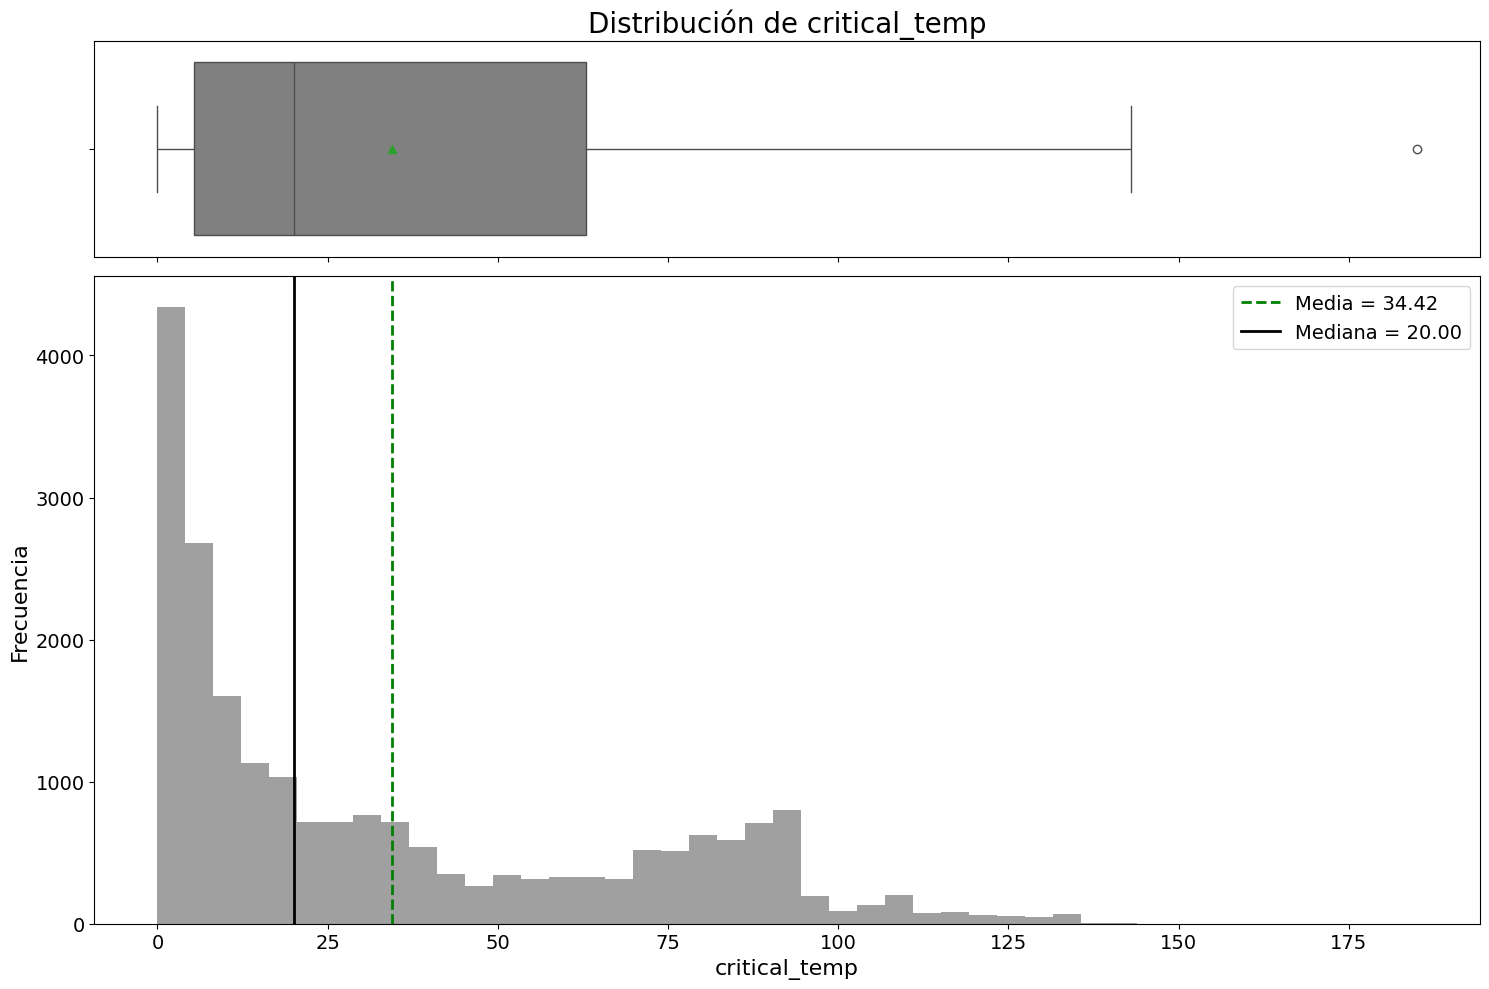
\includegraphics[width=0.75\linewidth]{critical_temp_distr.png}
    \caption{Distribución de la variable objetivo $T_c$.}
    \label{fig:critical_temp_distr}
\end{figure}

Como se observa en la Figura \ref{fig:critical_temp_distr}, la distribución de la temperatura crítica está sesgada a la derecha con la mayoría de los superconductores concentrados en el rango de temperaturas críticas entre $0\,K$ y $50\,K$. No obstante, la distribución se alarga hasta valores por encima de los $130\,K$, aunque se observa un claro descenso por encima de los $100\,K$. La distribución refleja la realidad experimental: los superconductores de alta temperatura crítica son excepcionales.

El resultado es un dataset desbalanceado, no por errores de muestreo, sino por la realidad física de este fenómeno. Este desequilibrio deberá tenerse en cuenta durante el modelado, ya que los algoritmos tenderán a sesgarse y ajustar mejor los compuestos con temperaturas críticas bajas.

Advertimos la presencia de un outlier con $T_c=185\,K$ que corresponde con el compuesto $H_2S$. No obstante, al tratarse de un outlier físico, no se elimina del conjunto de datos. Esta decisión se basa en que los modelos que se van a utilizar, basados en árboles de decisión, son robustos frente a la presencia de outliers.

\begin{figure}
    \centering
    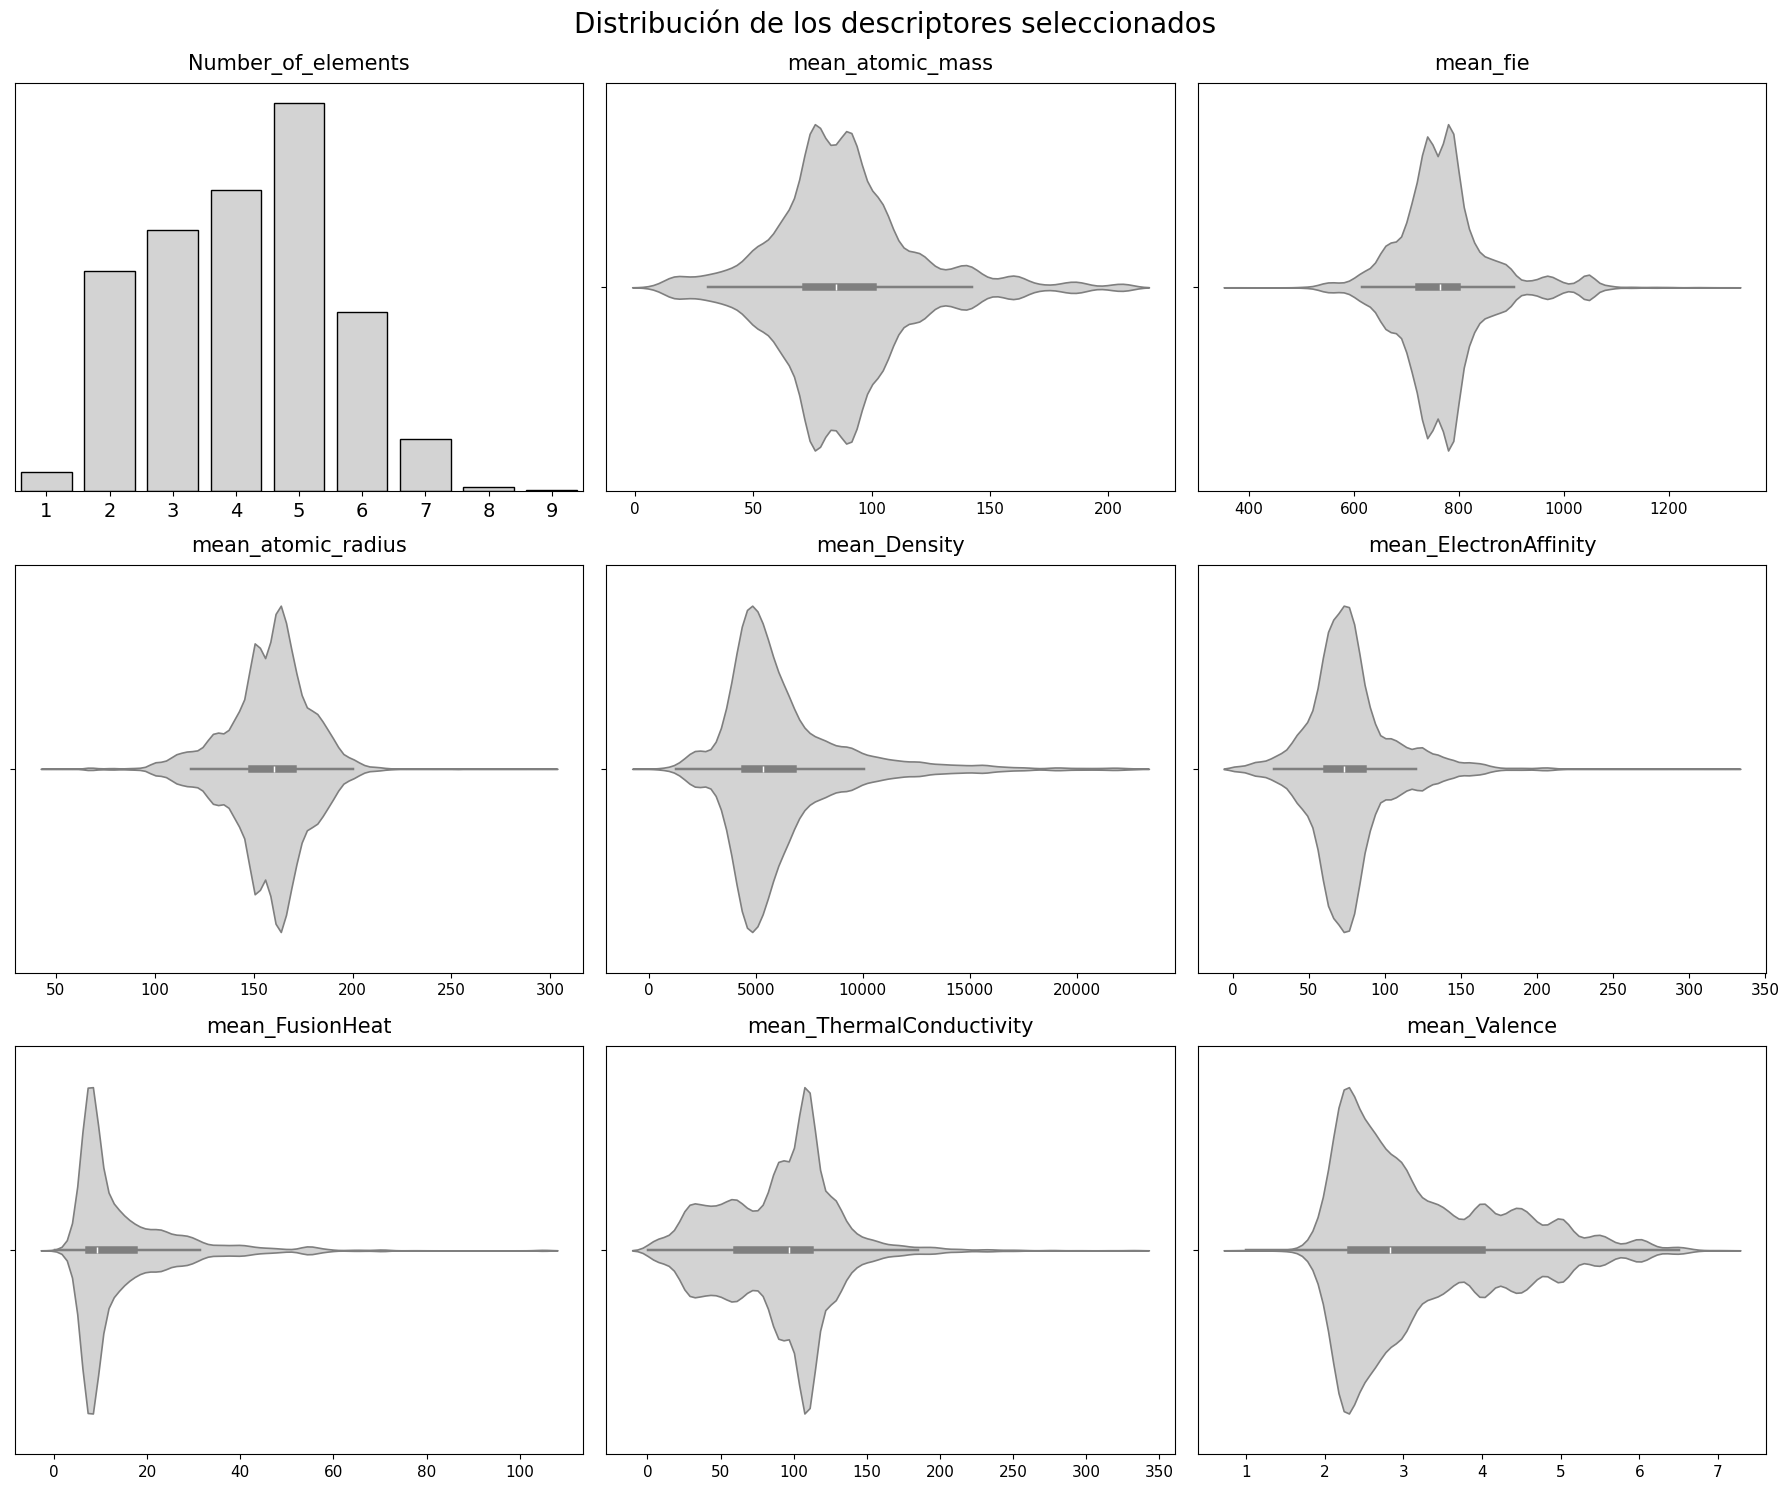
\includegraphics[width=0.75\linewidth]{univariante_distr.png}
    \caption{Distribuciones de los descriptores seleccionados para el análisis univariante.}
    \label{fig:univariante_distr}
\end{figure}

En la Figura \ref{fig:univariante_distr} podemos visualizar distribuciones con notables sesgos positivos, como es el caso de \textit{mean\_Density}, \textit{mean\_FusionHeat} y \textit{mean\_Valence}, hasta distribuciones más simétricas como  \textit{mean\_atomic\_mass}, \textit{mean\_fie} o \textit{mean\_ElectronAffinity}. En cambio, \textit{mean\_ThermalConductivity} y \textit{mean\_atomic\_radius} muestran un leve sesgo negativo.

En general, las variables presentan una dispersión considerable, con rangos amplios y la presencia de valores atípicos en la mayoría de los casos, especialmente en regiones superiores. Es importante notar que estos valores extremos no provienen de errores experimentales, sino de outliers físicos reales. Por ello se toma la decisión de mantenerlos, pues eliminarlos implicaría perder información física valiosa de comportamientos excepcionales, pero posibles.

\section*{Análisis bivariante}
En este punto nos centramos en las correlaciones entre descriptores y en particular, su relación con la variable objetivo \textit{critical\_temp}.

Este estudio permite observar cómo varía la temperatura crítica en función de las distintas propiedades atómicas y estructurales de los materiales y detectar tendencias y patrones físicos relevantes.

En primer lugar, se realiza una exploración visual de las relaciones de las variables explicativas de la familia \textit{mean\_*} y la variable objetivo. Este análisis lo hacemos a través de mapas de densidad, a través de los cuales podemos visualizar para qué valores se concentra una mayor cantidad de superconductores.

\begin{figure}
    \centering
    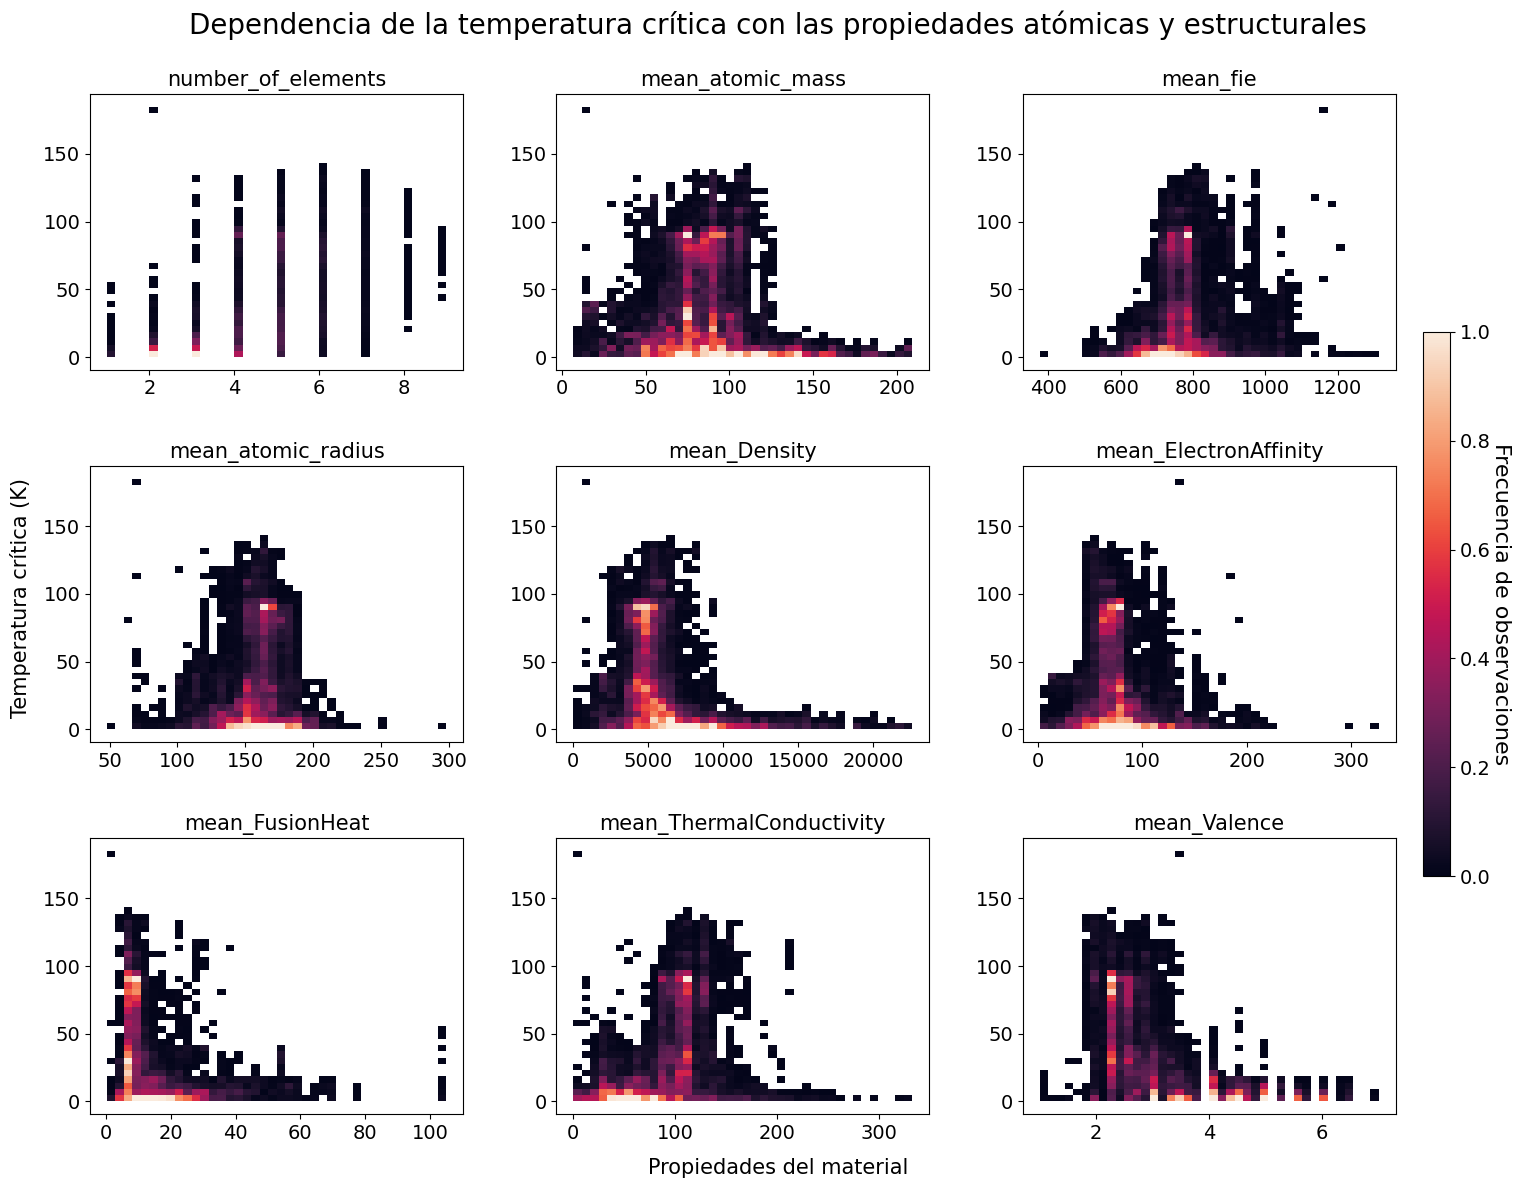
\includegraphics[width=0.75\textwidth]{bivariante_hist2d.png}
    \caption{Mapas de densidad para las relaciones entre los descriptores seleccionados y la variable objetivo.}
    \label{fig:bivariante_hist2d}
\end{figure}

En la Figura \ref{fig:bivariante_hist2d} se identifican zonas de concentración local de superconductores de alta temperatura. Esto ocurre generalmente en las regiones de mayor densidad de muestras (tanto de baja como de alta temperatura). Esto es, las temperaturas críticas altas se dan en subconjuntos específicos dentro de los rangos más comunes.

Para esta parte del análisis, en la que se pretende profundizar en qué propiedades resultan más determinantes en la variación de la temperatura crítica de los materiales superconductores, se ha decidido investigar la correlación de la variable objetivo con la familia \textit{range\_*}.

\begin{figure}
    \centering
    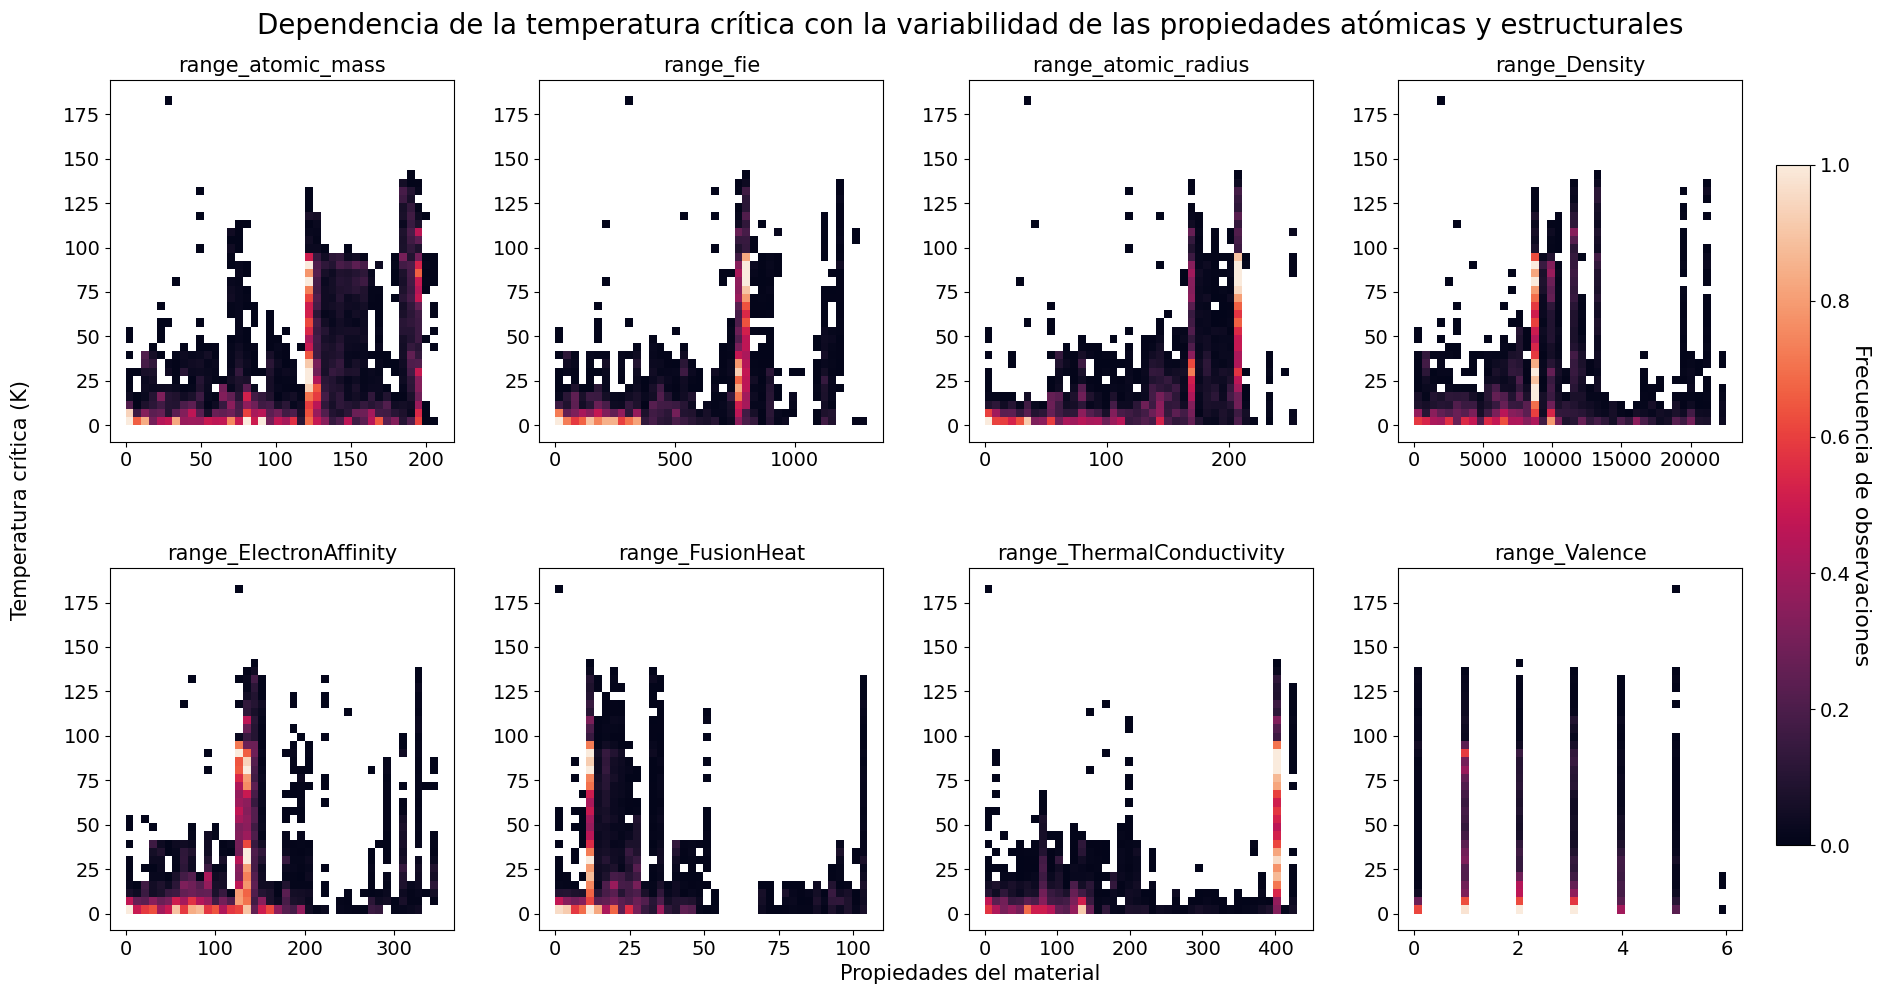
\includegraphics[width=0.75\textwidth]{bivariante_hist2d_var.png}
    \caption{Mapas de densidad para las relaciones entre los descriptores de la familia \textit{range\_*} y la variable objetivo.}
    \label{fig:bivariante_hist2d_var}
\end{figure}

En la Figura \ref{fig:bivariante_hist2d_var} se observan tendencias más marcadas que las vistas anteriormente para la familia \textit{mean\_*}. En particular, se aprecian intervalos concretos de estos descriptores que muestran una concentración elevada de superconductores de alta temperatura. Este comportamiento se refleja en \textit{range\_fie}, \textit{range\_ElectronAffinity} y, de forma más notoria, en \textit{range\_ThermalConductivity} que presenta una región relativamente limpia en la que se agrupan la mayoría de compuestos con temperaturas críticas elevadas, salvo algunas muestras aisladas fuera de ella.

Si bien este análisis permite identificar ciertos patrones en la relación entre las propiedades atómicas y estructurales y la temperatura crítica, no se identifican relaciones funcionales evidentes. Esto sugiere que el fenómeno superconductor depende de interacciones no lineales y multivariantes. Este comportamiento justifica la necesidad de emplear modelos de aprendizaje automático, capaces de capturar interacciones complejas entre múltiples variables.

Continuando nuestro análisis, adoptamos una perspectiva más estadística con el objetivo de explorar no solo la correlación existente entre cada una de las propiedades con la temperatura crítica, sino tambíen las posibles dependencias entre los propios predictores. Para ello calculamos la matriz de correlación de la familia \textit{mean\_*}.

\begin{figure}
    \centering
    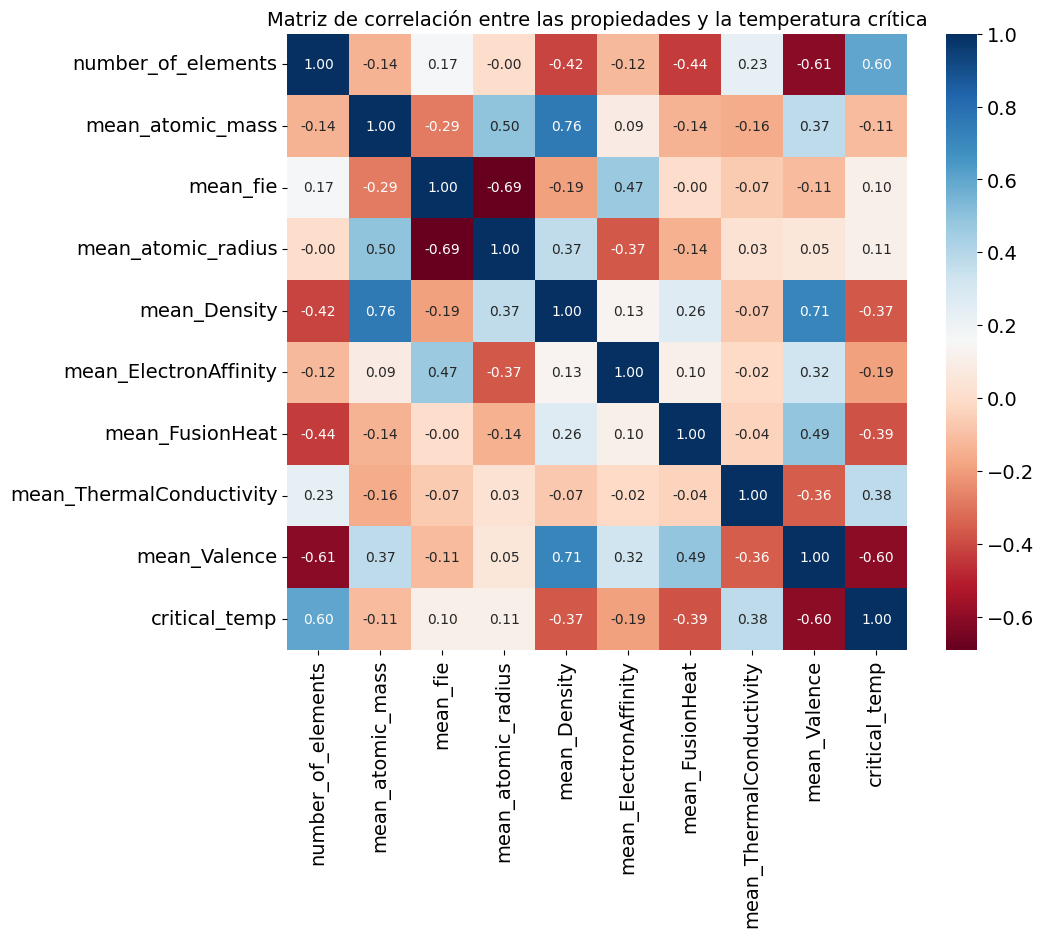
\includegraphics[width=0.6\textwidth]{matriz_mean.png}
    \caption{Matriz de correlación correspondiente a los descriptores seleccionados y la variable objetivo.}
    \label{fig:matriz_mean}
\end{figure}

En la Figura \ref{fig:matriz_mean} podemos advertir correlaciones entre las propiedades, todas ellas esperables desde el punto de vista físico-químico. Un ejemplo claro es la correlación positiva de \textit{mean\_atomic\_mass} con \textit{mean\_atomic\_radius} y \textit{mean\_Density} o la correlación negativa entre \textit{mean\_atomic\_radius} y \textit{mean\_fie} (a mayor tamaño del átomo, menor atracción sobre los electrones de valencia y menor energía de ionización).

Respecto a la variable objetivo, se observa correlación positiva notable con \textit{number\_of\_elements} y algo más moderada con \textit{mean\_ThermalConductivity}. Con \textit{mean\_Valence} se tiene una correlación negativa relativamente fuerte, y en menor medida con \textit{mean\_FusionHeat} y \textit{mean\_Density}. El resto de variables presentan correlaciones débiles con la temperatura crítica.

Dadas las relaciones observadas anteriormente para la familia \textit{range\_*}, consideramos también la obtención de su respectiva matriz de correlación, incluyendo también la variable objetivo.

\begin{figure}
    \centering
    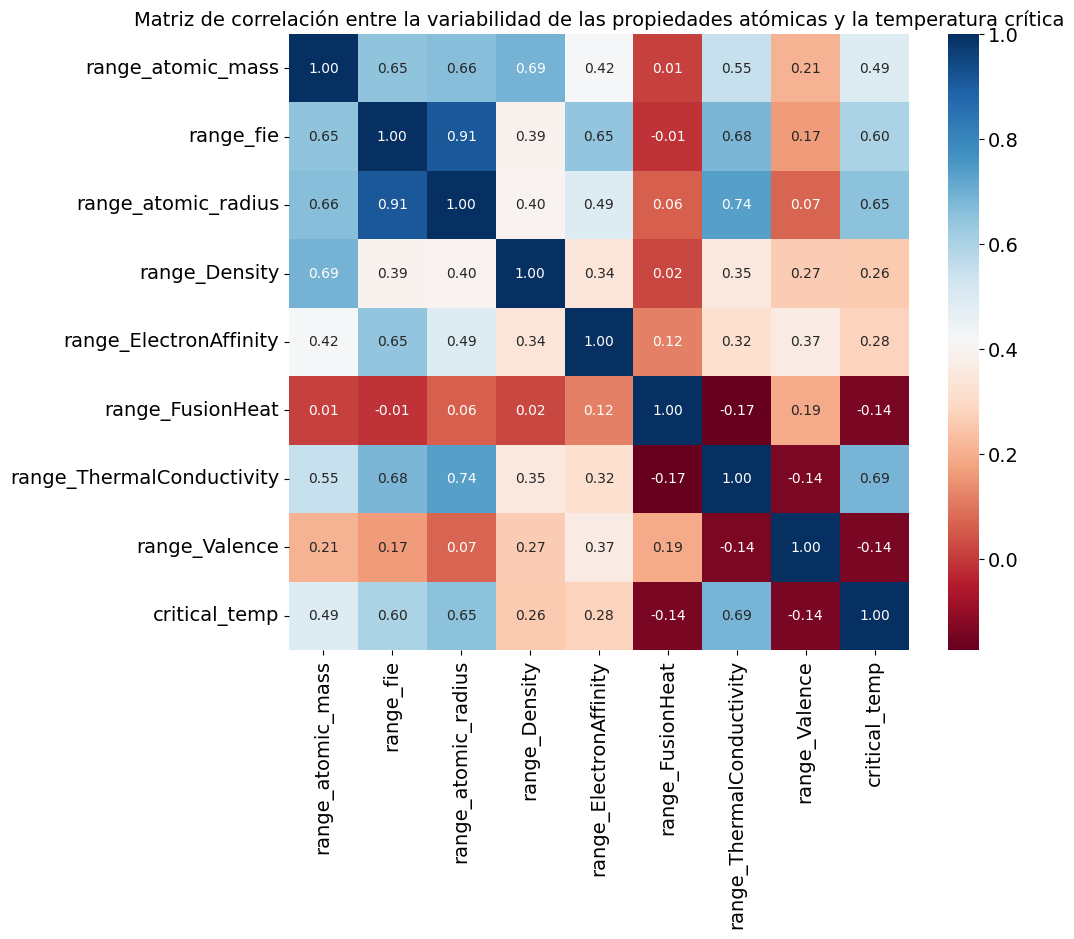
\includegraphics[width=0.6\textwidth]{matriz_range.png}
    \caption{Matriz de correlación correspondiente a los descriptores de la familia \textit{range\_*} y la variable objetivo.}
    \label{fig:matriz_range}
\end{figure}

Como podíamos esperar basándonos en la relación observada entre \textit{range\_ThermalConductivity} y la variable objetivo, obtenemos una correlación positiva considerable para este par. Son también destacables las correlaciones positivas de \textit{range\_fie} y \textins{range\_atomic\_radius} con \textit{critical\_temp}.


\begin{figure}
    \centering
    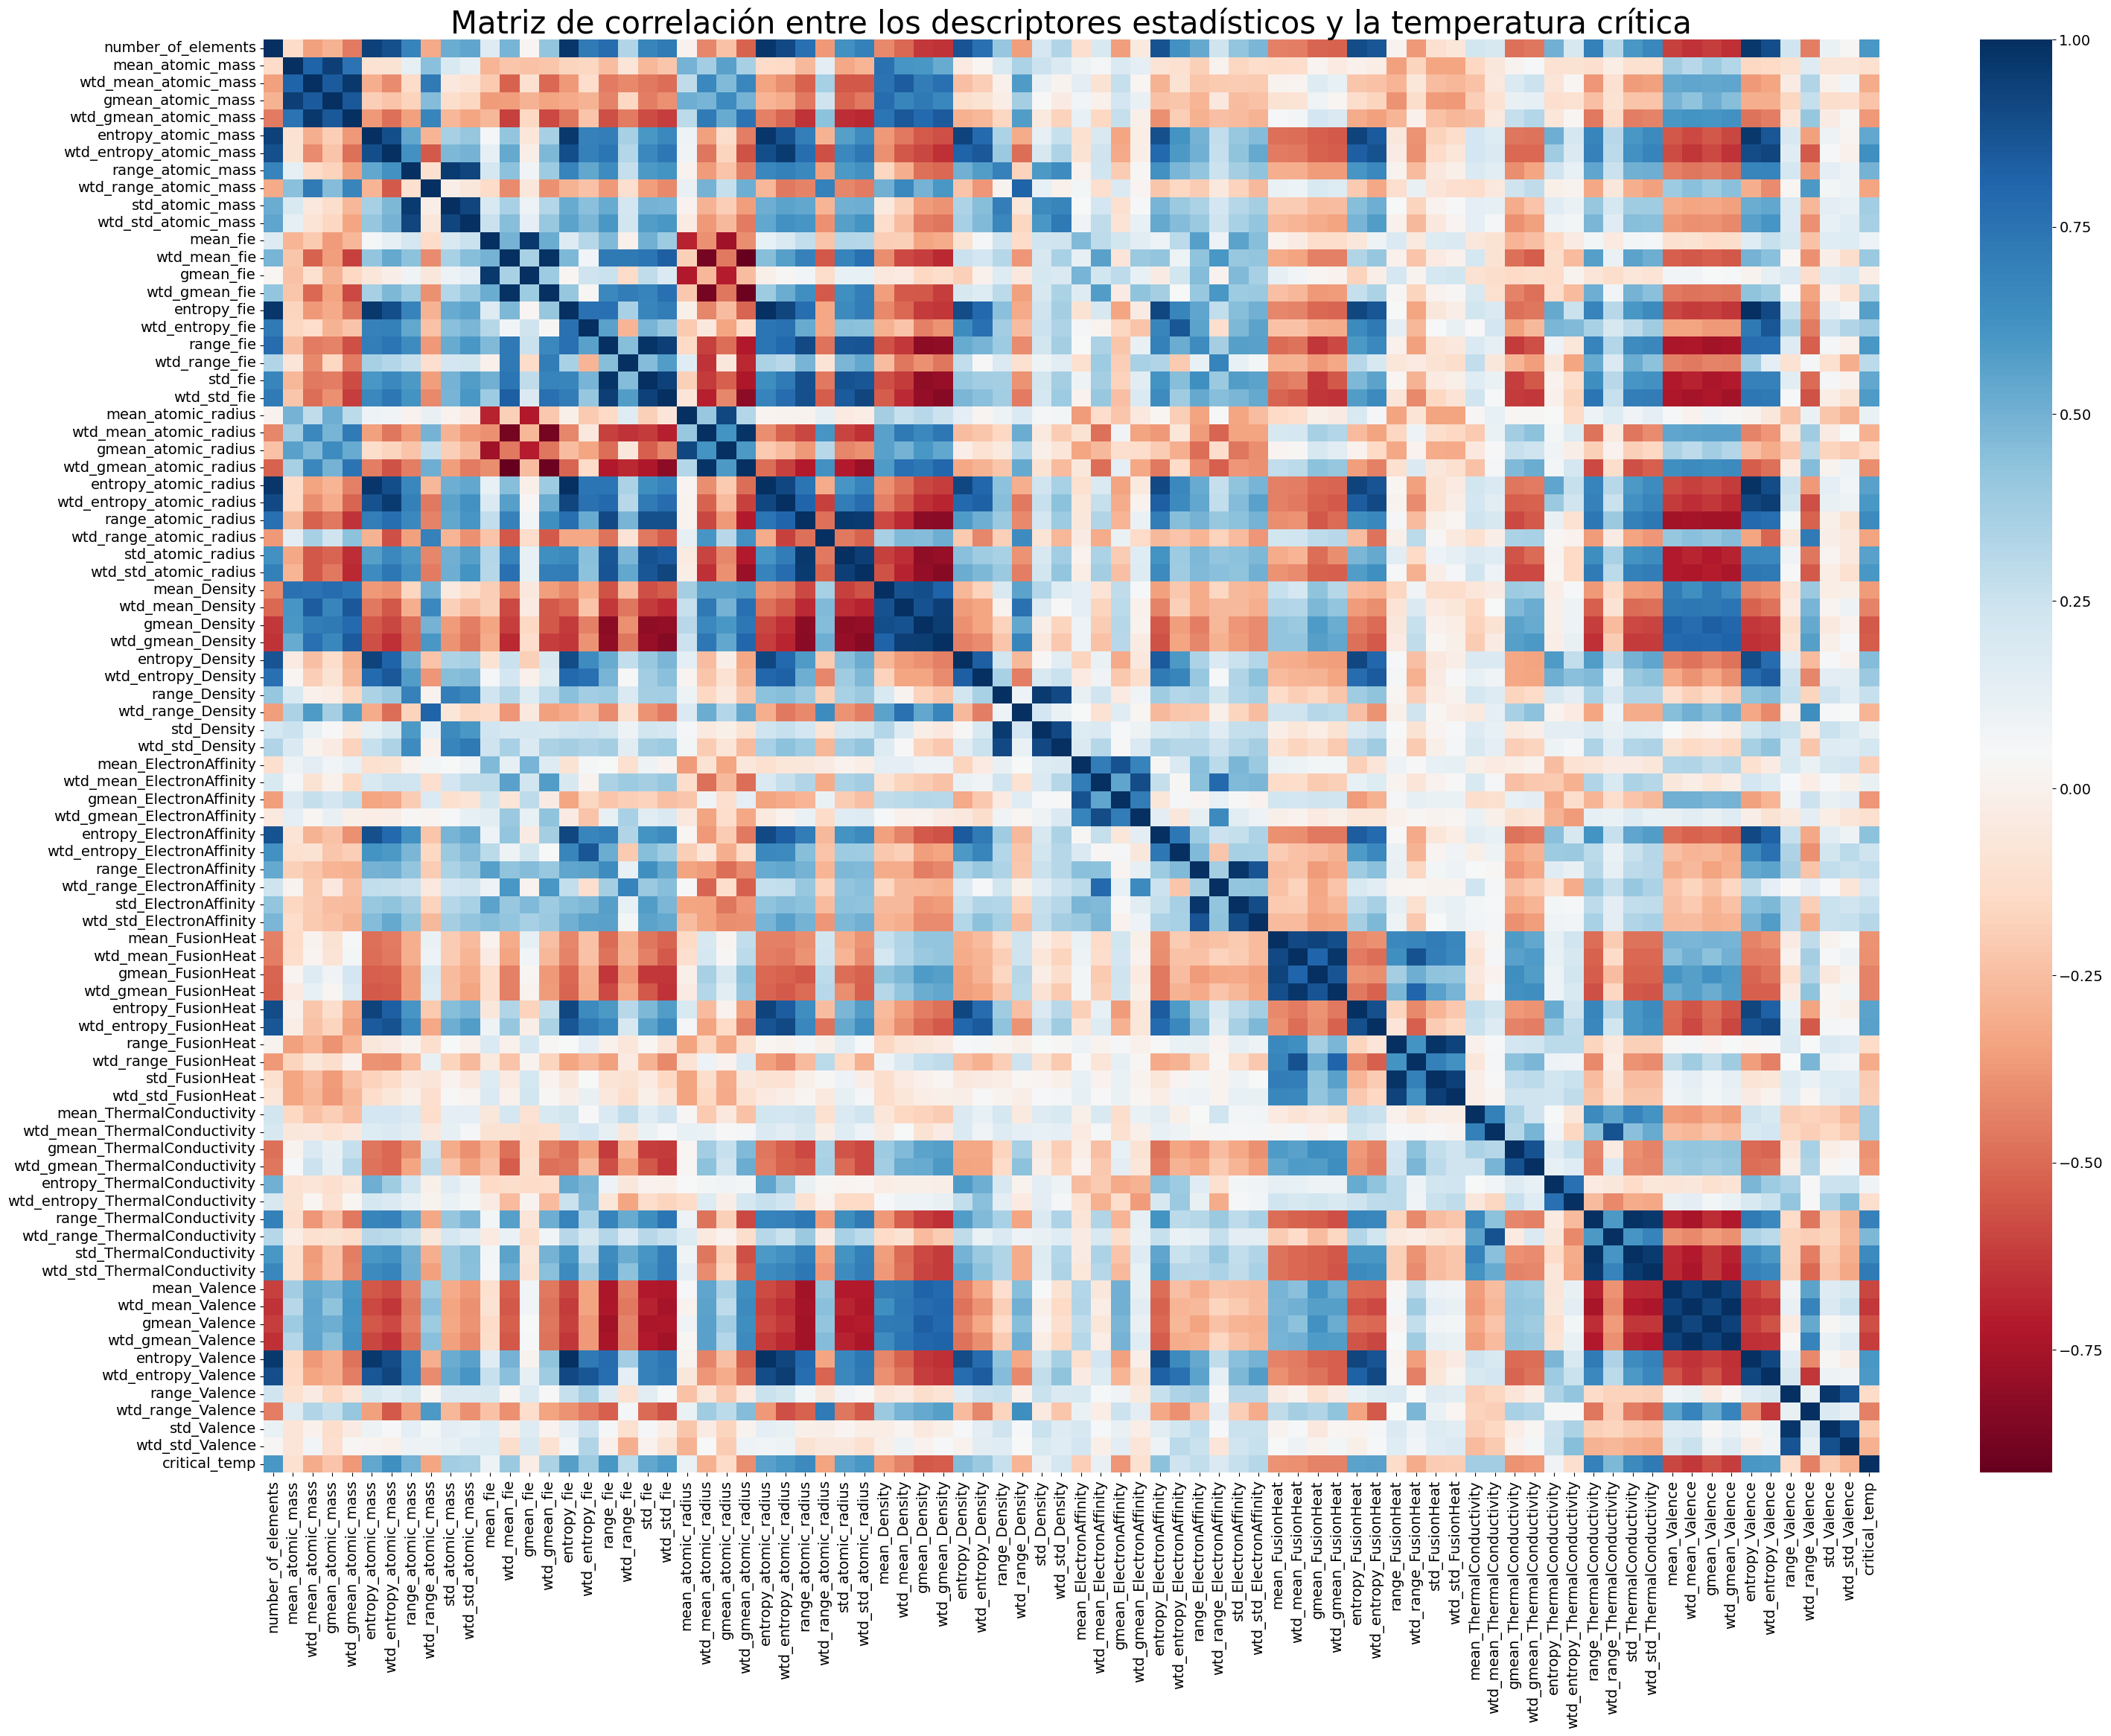
\includegraphics[width=0.6\textwidth]{matriz_Tot.png}
    \caption{Matriz de correlación completa. Se inclyen los 81 descriptores y la variable objetivo.}
    \label{fig:matriz_Tot}
\end{figure}

En la Figura \ref{fig:matriz_Tot} se incluye la matriz de correlación completa entre todas las variables del conjunto de datos. Como consecuencia de la gran cantidad de descriptores, se pierde detalle a nivel individal, pero podemos identificar patrones globales de dependencia. Vemos reforzadas las correlaciones ya observadas en el subconjunto analizado. No obstante, aparecen nuevas correlaciones interesantes, especialmente al considerar las familias \textit{range\_*} y \textit{std\_*}, lo que nos indica que, para ciertos materiales, la variabilidad en las propiedades atómicas es un factor relevante para determinar la temperatura crítica.

Este análisis también evidencia la alta multicolinealidad entre ciertas familias, como es el caso de \textit{mean\_*}, \textit{wtd\_mean\_*}, \textit{gmean\_*} y \textit{wtd\_gmean\_*}. No obstante, los modelos basados en árboles que se van a utilizar son capaces de gestionar internamente la redundancia y seleccionar las características más relevantes durante el entrenamiento.
\end{document}